\newpage
\pagestyle{fancy}
\fancyhead[RO]{\nouppercase{\textbf{Κεφάλαιο \ref{Ch:haz}} $|$ \textit{\nameref{Ch:haz}}}}
\fancyhead[LE]{\textit{\nameref{Ch:haz}} $|$ \nouppercase{\textbf{Κεφάλαιο \ref{Ch:haz}}}}
%\setcounter{page}{1}
%\setcounter{chapter}{0}

\chapter{Σεισμική Επικινδυνότητα}
\label{Ch:haz}
%\parencite{}
\section{Εισαγωγή}
Όπως ήδη ορίστηκε στην Υποενότητα \ref{Sbsec:Haz}, η σεισμική επικινδυνότητα είναι η πιθανότητα  να ξεπεραστεί ένα μέγεθος έντασης σε δεδομένη θέση. Από τα τρία μεγέθη της διακινδύνευσης, αυτό της επικινδυνότητας εξαρτάται εξ ολοκλήρου από τα φυσικά φαινόμενα, και δεν μπορεί να καθοριστεί από ανθρωπογενείς δράσεις. Άρα, η ακριβής πρόβλεψη των σεισμικών δράσεων αποτελή κρίσιμη παράμετρο σχεδιασμού.

Για να ποσοτικοποιηθεί η σεισμική δράση, χρειάζεται να μοντελοποιηθεί με κάποιον τρόπο, ο μηχανισμός δημιουργίας, μετάδοσης και εκτόνωσης των σεισμικών κυμάτων. Η ποσοτικοποίηση αυτή, ακολουθεί δύο βασικές μεθόδους ανάλυσης.

Η πρώτη είναι η αιτιοκρατική μέθοδος, η οποία αποσκοπεί να υπολογίσει κάποιο μέγιστο μέγεθος έντασης, αναγνωρίζοντας χαρακτηριστικές δράσεις της μελετούμενης περιοχής. Αιτιοκρατικά οφείλεται να μελετούνται οι κατασκευής πολύ μεγάλου χρόνου ζωής, όπου ελλείπουν πολύ μακροχρόνια ιστορικά δεδομένα σεισμικότητας, και μία στατιστική προσέγγιση είναι δυσχερέστερη.

Η δεύτερη είναι η πιθανοτική μέθοδος \parencite{Cornell, McGuire}, κατά την οποία ορίζονται κατανομές πιθανότητας εμφάνισης και μεγεθών σεισμών για τους σεισμούς, σχέσεων εξασθένισης και τοπικών εδαφικών συνθηκών ώστε να προκύψει η συσχέτιση των μεγεθών έντασης με αντίστοιχες πιθανότητες.

%Ακόμη, οι σεισμοί παραμένουν κατεξοχήν ένα χωροχρονικώς αβέβαιο φαινόμενο, και η ακριβής πρόβλεψη αυτών παραμένει αδύνατη για τα θνητά όντα.

\section{Ορισμοί}
Ο σεισμός είναι το φυσικό φαινόμενο κατά το οποίο δημιουργείται ένα σεισμικό κύμα σε μία πηγή που εξαπολύει σεισμική ενέργεια. Αφού το κύμα ακολουθήσει μία διαδρομή και μετασχηματιστεί από τις τοπικές εδαφικές συνθήκες μίας γεωγραφικής θέσης, δίνει στην θέση αυτή κάποια απόκριση. Οι ορισμοί των επιμέρους αναφερόμενων όρων επεξηγούνται στην παρούσα ενότητα.

\subsection{Κύματα}
\label{sbs:Waves}
Η σεισμική ενέργεια μεταδίδεται από το υπέδαφος στην επιφάνεια της Γης μέσω κυμάτων. Αυτά τα κύματα χωρίζονται στην σεισμολογία σε χωρικά και επιφανειακά.

Τα χωρικά κύματα είναι εκείνα που έχουν προέλευση κάποια πηγή, και ταξιδεύουν μέσα στον χώρο (τρεις διαστάσεις), και χωρίζονται με την σειρά τους στα διαμήκη και τα εγκάρσια. Τα επιφανειακά από την άλλη, προκύπτουν από τον μετασχηματισμό των χωρικών κυμάτων μέσα στο έδαφος, και ταξιδεύουν στην επιφάνεια της Γης (δύο διαστάσεις), ενώ μεταδίδονται με μικρότερη ταχύτητα των χωρικών.

Από τα χωρικά τμήματα, τα διαμήκη (ή πρωτεύοντα, P) είναι αυτά που προκαλούν κίνηση κατά την διεύθυνση μετάδοσης των. Έτσι στην μετάδοση αυτών των κυμάτων, το έδαφος συστέλεται και διαστέλεται αξονικά. Στις επιφανειακές κατασκευές, τα κύματα P προκαλούν κατακόρυφες δράσεις, και καθώς οι περισσότερες κατασκευές είναι υπερδιαστασιολογημένες ως προς τα φορτία βαρύτητας, σπάνια η δράση τους είναι σημαντική. Υπάρχουν εξαιρέσεις όπου οι κατακόρυφες δράσεις είναι κρίσιμες, ειδικότερα σε συνδυασμό με άλλες δράσεις, αλλά οι σήραγγες δεν αποτελούν τέτοια περίπτωση.

Τα εγκάρσια κύματα (ή δευτερεύοντα, S), ακολουθούν χρονικώς τα διαμήκη, και η κίνηση που προκαλούν στο έδαφος, είναι κάθετη στην διεύθυνση μετάδοσης των. Επομένως οι παραμορφώσεις που προκαλούν είναι παράλληλες με την επιφάνεια του εδάφους και, στην συντριπτική πλειοψηφία των σεισμικών δράσεων, αποτελούν την κρίσιμη δράση.

Καθώς οι περισσότερες κατασκευές ορίζονται σε δύο κάθετους μεταξύ τους άξονες, ευνοεί η ανάλυση των εγκαρσίων κυμάτων σε δύο διευθύνσεις. Έτσι ορίζονται τα κύματα SV και SH. Στην συγκεκριμένη εργασία θεωρείται η διεύθυνση SH αυτή κατά μήκος της σήραγγας, ενώ η διεύθυνση H αυτή κατά πλάτος της διατομής. Η συνεισφορά της σεισμικής δράσης κατά τον άξονα της σήραγγας είναι σημαντικός παράγοντας στην σεισμική διακινδύνευση των σηράγγων, αλλά απαιτεί τρισδιάστατη σεισμική ανάλυση και προτιμήθηκε να αναλυθεί η δράση μόνο των SV κυμάτων.


\begin{figure}[ht]
	\centering
	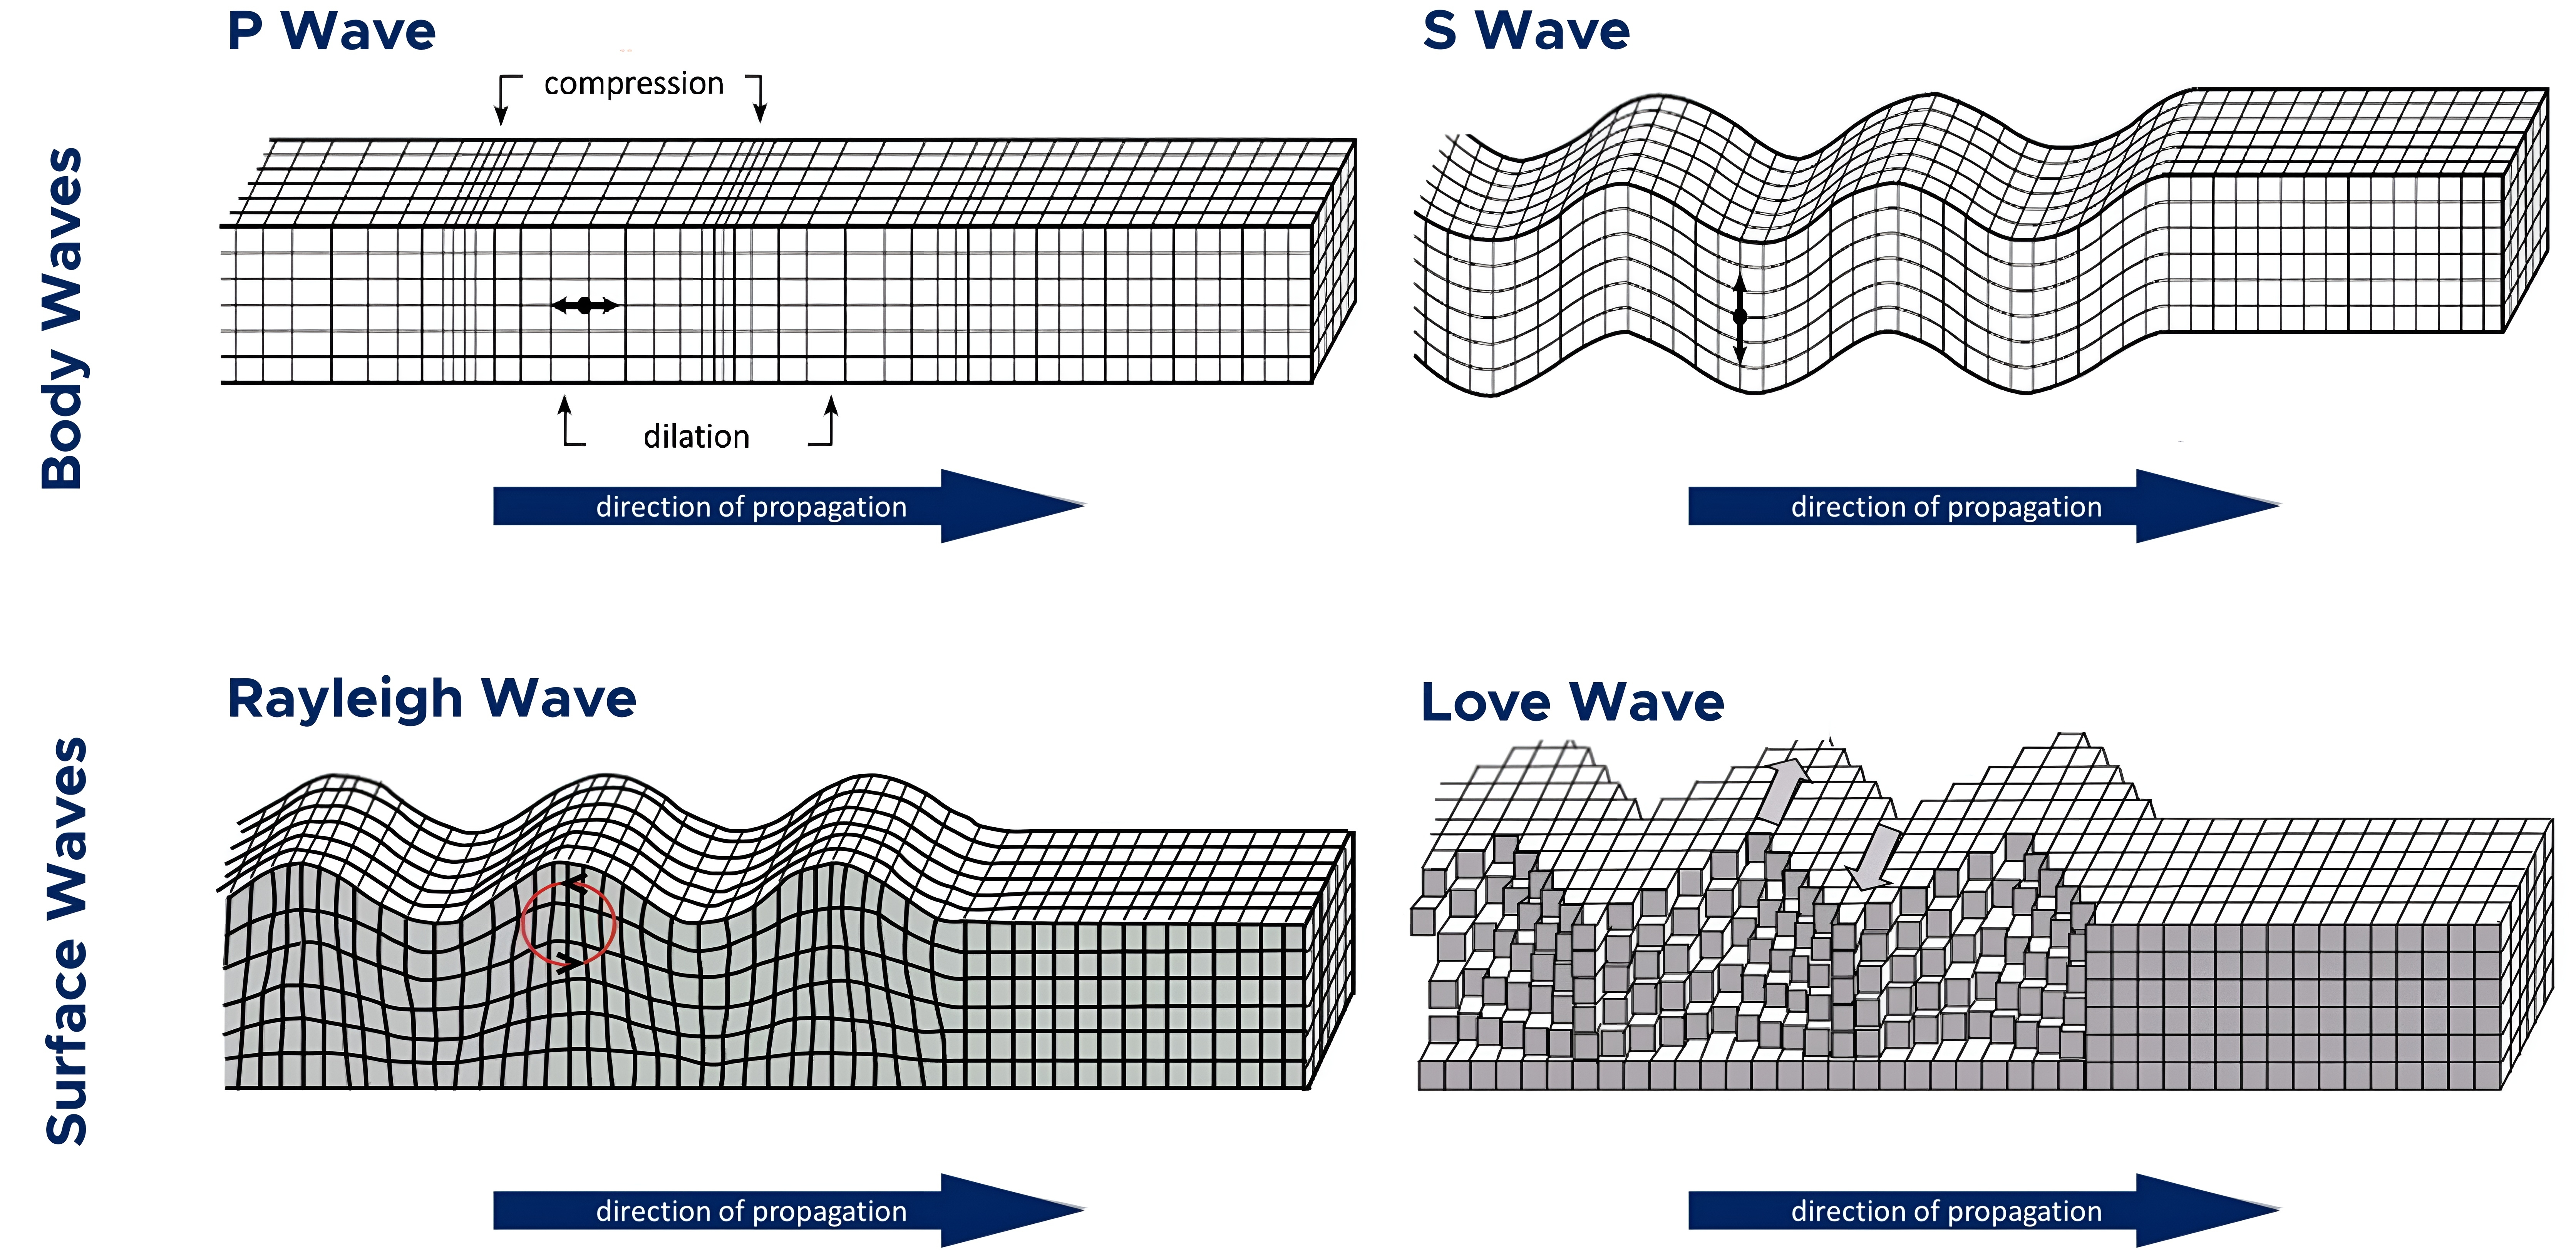
\includegraphics[width=1.03\linewidth]{figures/hazard/waves.jpeg}
	\caption{Τύποι Σεισμικών Κυμάτων (Πηγή: \href{https://commons.wikimedia.org/wiki/File:Overview_Seismic_Waves.jpg}{LukeTriton κ.α.})}
	\label{fig:waves}
\end{figure}

Τέλος, τα επιφανειακά κύματα είναι σύνθετα και μπορεί να έχουν πολλές μορφές, αλλά οι δύο βασικότερες είναι τα Rayleigh και Love. Καθώς τα επιφανειακά κύματα μεταδίδονται σε δύο διαστάσεις, ενώ τα χωρικά σε τρεις, τα πρώτα εξασθενίζονται με χαμηλότερο ρυθμό και έτσι μπορούν να καταγραφούν υψηλές αποκρίσεις σε πολύ μεγάλες αποστάσεις. \parencite{Stein}

Στο Σχήμα \ref{fig:waves} φαίνονται οι μορφές των βασικών κυμάτων.

\subsection{Πηγές}
\label{sbs:Source}

Η δημιουργία των σεισμών συμβαίνει από τις χαρακτηριζόμενες πηγές της Γης, οι οποίες έχουν είτε την μορφή ρήγματος, είτε ηφαιστειακή προέλευση.

Σημαντικές ηφαιστειακές πηγές δεν υπάρχουν στην βόρεια Ελλάδα, οπότε εστιάζονται οι τύποι των ρηγμάτων.

Τα ρήγματα αντίστοιχα, χωρίζονται σε δύο επί μέρους κατηγορίες, όπου είναι οι τεκτονικές κινήσεις και τα επιφανειακά ρήγματα.

Οι σεισμοί που προέρχονται από τις κινήσεις των τεκτονικών πλακών συμβαίνει από την αλληλεπίδραση δύο πλακών. Η καταβύθιση μία ωκεάνιας πλάκας κάτω από μία ηπειρωτική οδηγεί σε θλιπτικές τάσης μεταξύ των πλακών και μεγάλη απελευθέρωση ενέργειας. Η αλληλεπίδραση των δύο πλακών σε μεγάλα βάθη προκαλεί επίσης σεισμούς, αλλά με μικρότερη κλίμακα. Αντίστοιχα, η απομάκρυνση μίας ωκεάνιας πλάκας από μια ηπειρωτική δημιουργεί εφελκυστικές τάσεις, ενώ η παράλληλη κίνηση πλακών μπορεί να έχει τα μεγαλύτερα μήκη και τεράστια απελευθεύρωση ενέργειας, από συγκέντρωση διατμητικών τάσεων.

Τα επιφανειακά κύματα εμφανίζονται εντός του μανδύα της Γης, και μπορεί να είναι κανονικά, ανάστροφα ή διατμητικά (ή μεικτού τύπου). Τα κανονικά ρήγματα είναι εκείνα τα οποία οφείλονται σε εφελκυστικές τάσεις, και η κίνηση κατά το ρήγμα προκαλεί καταβύθιση του ποδός. Αντίθετα, τα αντίστροφα ρήγματα οφείλονται σε θλιπτικές τάσεις, όπου ο πους ανυψώνεται υπέρ της στέψης του ρήγματος. Τέλος τα διατμητικά ρήγματα προκαλούν τις δύο πλευρές να κινούνται παράλληλα, χωρίς την ανύψωσωη ή την καταβύθιση κάποιου σημείου. \parencite{YuHu}

Η ενεργοποίηση των ρηγμάτων, μπορεί να εξηγηθεί από την θεωρία ελαστικής ανάπαλσης \parencite{Reid}. Στην συγκεκριμένη θεωρία, προτείνεται ότι η γέννεση των σεισμών, πραγματοποιείται λόγω μακροχρόνιας συγκέντρωσης τάσεων σε ένα ρήγμα. Για επαρκώς δύσκαμπτη διεπιφάνεια, οι διατμητικές τάσεις αυξάνονται μέχρι να ξεπεραστεί η επιφανειακή τριβή του ρήγματος και να υπάρξει ταχεία μετακίνηση αυτού. Αυτή η ξαφνική απελευθέρωση τάσεων είναι που προκαλεί, σύμφωνα με την συγκεκριμένη θεωρία, τους σεισμούς στα ρήγματα.

Πλέον επικρατούν και άλλες ερμηνείες των φαινομένων, εξηγώντας αναλυτικότερα τα αίτια που οδηγούν στην μετακινήση ως το φαινόμενο τριβής-ολίσθησης (stick-slip effect) \parencite{Brace} και τον μηχανισμό ασεισμικής συμπεριφοράς ορισμένων ρηγμάτων \parencite{Wang}.

% Τα περί πηγών ίσως πρέπει να μπουν μετά για την μοντελοποίηση της πηγής, δεν ξέρω
%Προσομοίωση πηγών
%Σημειακές, γραμμικές τρισδιάστατες
%MFD

Στην προσομοίωση των ρηγμάτων ως πηγές, αυτά περιγράφονται σύμφωνα με την γεωμετρία τους αλλά και την συχνότητα εμφάνισης σεισμών συγκεκριμένου μεγέθους. Ο ετήσιος αριθμός ορισμένων μεγεθών ορίζεται από κάποια στατιστική κατανομή. Μία συνηθισμένη σχέση που χρησιμοποιείται, είναι αυτή των Gutenberg και Richter, όπου ο λογάριθμος του αριθμού των σεισμών που ξεπερνούν ένα μέγεθος, αντιστοιχεί γραμμικά σε αυτό όπως φαίνεται στην Εξίσωση \ref{eq:GR} \parencite{GR}.

\begin{equation}
	\log{N} = a - b M
	\label{eq:GR}
\end{equation}

\subsection{Διαδρομή}
Αφού απελευθερωθεί ένα κύμα στην πηγή, ακολουθεί η μετάδοση του στον χώρο. Η διαδρομή που θα ακολουθήσει ένα κύμα έχει μεγάλη σημασία καθώς η ενέργεια τους εξασθενίζεται γρήγορα όσο μακρύτερα κινούνται.

Το μέγεθος έντασης που θα δώσει μία σεισμική ρήξη σε μία θέση μπορεί να είναι εντελώς αμελητέα για μεγάλες θέσεις, και έτσι -κυρίως για τα P και S κύματα- επομένως και ο συνυπολογισμός των ίδιων των πηγών εξαρτάται από την απόσταση τους με την θέση.

Αντίστοιχα, ένα ρήγμα μπορεί να απελευθερώνει έναν σεισμό με συγκεκριμένη κατεύθυνση, επηρεάζοντας μία εγγύτερη θέση περισσότερο από μία μακρύτερη λόγω αυτού του φαινομένου.


\subsection{Τοπικές Εδαφικές Συνθήκες}
Με την άφιξη του σεισμικού κύματος κοντά στην θέση μελέτης, η τελευταία επιρροή πάνω στο κύμα είναι αυτή των τοπικών εδαφικών συνθηκών.

Καθώς στην επιφάνεια του εδάφους οι εδαφικές στρώσεις είναι τυπικά μαλακότερες, ένα κύμα που καταφτάνει σε αυτές, μπορεί να εμφανίσει έντονα φαινόμενα διάθλασης και ανάκλασης, παγιδεύοντας τα κύματα κοντά στην επιφάνεια και επηρεάζοντας σημαντικά την ένταση, την διάρκεια και το συχνοτικό περιεχόμενο της επιφανειακής απόκρισης.

Ακόμα, είναι δυνατό μία ισχνή απόκριση σε βράχο, κοντά στην θέση μελέτης, να ενισχυθεί σε τέτοιον βαθμό που να αποτελέσαι ισχυρή εδαφική κίνηση. Μία τέτοια περίπτωση είναι ο σεισμός του Μιχοατσάν το 1985, όπου προκλήθηκε περίπου 400 χιλιόμετρα μακρύτερα της πόλης του Μεξικού. Καταγραφές από το πανεπιστήμιο της πόλης, οι οποίες λήφθησαν σε σχεδόν οιονεί βραχώδες υπόβαθρο δείχνουν σημαντική εξασθένιση μετρώντας μέγιστη εδαφική επιτάχυνση περί τα $0.03g$. Αντίθετα, στο κέντρο της πόλης όπου επικρατούν πολύ μαλακές λιμναίες αποθέσεις μέχρι και τριάντα μέτρα πάχους, η μέτρηση φτάνει τα $0.167g$  με κυρίαρχη ιδιοπερίοδο στα $2\;sec$ \parencite{Mex}.

Για αυτούς τους λόγους, είναι πολύ σημαντική η εκτίμηση των τοπικών εδαφικών συνθηκών, ώστε να υπολογιστεί η συμπεριφορά του εδάφους σε σεισμικά γεγονότα.

Υπάρχουν αρκετές παράμετροι που δείχνουν την επιρροή των τοπικών εδαφικών συνθηκών, όπως η τοπογραφία, η σειρά των στρώσεων και άλλα, όμως, ένας απλός τρόπος για κατηγοριοποίηση είναι η μέση ταχύτητα μετάδοσης των διατμητικών κυμάτων, για τα πρώτα τριάντα μέτρα εδαφικών αποθέσεων.

\begin{equation}
	V_{s30} = \dfrac{30}{\sum_{i=1}^{30} t_i/V_{si}}
	\label{eq:vs30}
\end{equation}

\begin{equation}
	V_{s30} = \dfrac{\sum_{i=1}^{30} V_{si} \cdot t_i}{30}
	\label{eq:avevs}
\end{equation}

Η συγκεκριμένη παράμετρος υπολογίζεται από την Εξίσωση \ref{eq:vs30}, όπου $t_i$ και $V_{si}$ το πάχος και η ταχύτητα μετάδοσης διατμητικών κυμάτων στην κάθε στρώση ανίστοιχα, και επιτρέπει μία γενική εποπτεία για την σεισμική συμπεριφορά του εδάφους κοντά στην επιφάνεια.

Η Εξίσωση \ref{eq:vs30} \parencite{NEHRP} αναφέρεται ως η μέση ταχύτητα διάδοσης διατμητικών κυμάτων, αλλά δεν δίνει ισοδύναμη μέση τιμή όπως στην Εξίσωση \ref{eq:avevs} όσο μία βεβαρυμένη μορφή αυτής. Το πηλίκο του πάχους με την ταχύτητα μετάδοσης σε κάθε στρώση, δίνει περισσότερο βάρος στις στρώσεις χαμηλότερων ταχυτήτων.

Μία τέτοια προσομοίωση των φυσικών φαινομένων ενδέχεται να έχει μεγαλύτερη ακρίβεια από μία απλή μέση τιμή, καθώς σε μία ομοιόμορφη στρωματογραφία η τιμή θα είναι σχεδόν ίδια με την μέση, ενώ σε εντόνως ανομοιόμορφη στρωματογραφία θα επικρατούν οι χαμηλότερες ταχύτητες. Ο λόγος που αυτό συμβαίνει είναι ότι οι πολύ υψηλές ταχύτητες μεταβάλλουν ελάχιστα τα μεταφερόμενα κύματα, ενώ οι χαμηλές μπορεί να εμφανίζουν πολλά φαινόμενα ανάκλασης, διάθλασης και απόσβεσης των κυμάτων, δίνοντας μεγαλύτερη έμφαση στις χαμηλές ταχύτητες.

Ο ίδιος τύπος μπορεί να χρησιμοποιηθεί αντί για την ταχύτητα μετάδοσης διατμητικών κυμάτων και για τιμές αντοχής των στρωμάτων αστράγγιστης διατμητικής αντοχής και αριθμού χτύπων $N_{30,\;i}$. Σε μία τέτοια περίπτωση ίσως να φαίνεται και σαφέστερα η σημασία του, καθώς στην περίπτωση παραλλήλως παρατεταγμένων υλικών, η συνολική αντοχή των εξαρτάται από την χαμηλότερη.

Φυσικά, μία τέτοια προσομοιώση λαμβάνει ορισμένες παραδοχές που μπορεί να παραπλανήσουν από την φύση, όπως είναι η παρουσία μίας πολύ λεπτής στρώσης χαμηλής ταχύτητας, ή το γεγονός ότι αγνοείται η σειρά των στρώσεων, όπου η εμφώλευση μίας στρώσης χαμηλής ταχύτητας ανάμεσα σε δύο υψηλής επηρεάζει τις τελικές αποκρίσεις. Η μελέτη τέτοιων υποπεριπτώσεων όμως είναι ανώφελη, καθώς η χρήση του $V_{s30}$ είναι καθαρώς η κατηγοροιοποίηση εδαφικών κατατομών και η στατιστική επεξεργασία των, και όχι ο καθέ αυτό υπολογισμός αποκρίσεων.

\section{Αιτιοκρατική Ανάλυση}

\subsection{Μεθοδολογία}

Πριν την ραγδαία ανάπτυξη των ηλεκτρονικών υπολογιστών, η αιτιοκρατική μέθοδος ήταν η μοναδική μέθοδος που μπορούσε να αποδώσει σεισμική επικινδυνότητα. Η μεθοδολογία μπορεί να χωριστεί σε τέσσερα βασικά βήματα \parencite{Reiter}.

Πρώτον, χρειάζεται να οριστούν οι κατάλληλες πηγές, οι οποίες μπορούν να αποδώσουν σημαντικούς σεισμούς στην μελετούμενη περιοχή. Όπως ορίσθηκε στην Υποενότητα \ref{sbs:Source}, οι πηγές πρέπει να χαρακτηρίζονται από την γεωμετρία και το σεισμικό δυναμικό που διαθέτουν.

Έπειτα, επιλέγεται για κάθε πηγή η απόσταση της από την εκάστοτε θέση μελέτης. Αυτή η απόσταση μπορεί να οριστεί ως επικεντρική, υποκεντρική ή κάπως αλλιώς, και συνήθως θα επιλεγεί η μικρότερη δυνατή.

Αφού οριστούν τα γεωμετρικά χαρακτηριστικά, ως τρίτο βήμα πρέπει να οριστεί η κυρίαρχη σεισμική κίνηση. Η επιλογή γίνεται σε σχέση με κάποιο μέγεθος έντασης, και λαμβάνοντας υπ' όψιν τους αναμενόμενους σεισμούς που μπορεί να δημιουργήσει η κάθε πηγή για την απόσταση που απέχει από την θέση.

Τέλος, η επικινδυνότητα στην θέση μελέτης υπολογίζεται από τα ανωτέρω δεδομένα. Όλοι οι υπολογισμοί στην αιτιοκρατική μέθοδο γίνονται με εμπειρικές ή αναλυτικές σχέσεις.

\subsection{Σκοπιμότητα Μεθόδου}
Από τα ανωτέρω, είναι σαφές ότι η αιτιοκρατική μέθοδος δεν συσχετίζει το μέγεθος έντασης με κάποια πιθανότητα στα αποτελέσματα της, τουλάχιστον όχι άμεσα. Έτσι, η βασικότερη διαφορά της αιτιοκρατικής από την πιθανοτική μέθοδο, είναι πως η αιτιοκρατική αποτελεί μία απλή και αναλυτική λύση για τον προσδιορισμό του δυσχερέστερου δυνατού ενδεχόμενου σε μία θέση, ενώ η πιθανοτική μία περίπλοκη, υπολογιστικά βεβαρυμένη και στατιστική μέθοδο. Αυτό είναι που την θέτει πολύ χρήσιμη για έργα μακρού χρόνου ζωής.

Φυσικά, η αιτιοκρατική μέθοδος έχει τους περιορισμούς της, καθώς περιλαμβάνει αρκετή επιστημονική ερμηνεία των δεδομένων και η εφαρμογή της απαιτεί αρκετές υποκειμενικές επιλογές, και τα αποτελέσματα που παράγει μπορεί να μην είναι ακριβή, αφού η σεισμικότητα αλλάζει στις περιοχές με τα χρόνια και το μέγιστο δυνατό μέγεθος μιας πηγής δεν γίνεται να εξακριβωθεί ποτέ με βεβαιότητα.

%\subsection{Σεισμικότητα Θεσσαλονίκης}
%\parencite{Papaz}

\section{Πιθανοτική Ανάλυση}
\subsection{Πλαίσιο Εφαρμογής}
Η εκτίμηση της σεισμικής επικινδυνότητας στην συγκεκριμένη έρευνα, πραγματοποίηθηκε με εφαρμογή πιθανοτικής ανάλυσης για την παραγωγή καμπύλων επικινδυνότητας σε χαρακτηριστικές θέσεις του έργου, και μέσης επικινδυνότητας κατά μήκος του.

Η μέση επικινδυνότητα, ορίστηκε για σεισμικά γεγονότα περιόδου επαναφοράς, 125, 600 και 2500 ετών, σύμφωνα με τον υπό εξέταση αναθεωρημένο Ευρωκώδικα 8, για οριακές καταστάσεις μηδενικών, σοβαρών και ολοκληρωτικών ζημιών της κατασκευής και θεωρώντας τις σήραγγες ως έργο σημασίας κατηγορίας 3.

Για την πραγματοποίηση των αναλύσεων χρησιμοποίηθηκε το OpenQuake Engine του Global Earthquake Model \parencite{Pagani} το οποίο αποτελεί μία εύχρηστη εφαρμογή εκτέλεσης PSHA. Πλεονέκτημα στην χρήση της συγκεκριμένης εφαρμογής αποτελούν η προσαρμοστικότητα στα εισαγόμενα δεδομένα, ο μεγάλος αριθμός από διαθέσιμες σχέσεις και η υψηλή αξιοπιστία που έχει λόγω της ευρείας χρήσης που λαμβάνει.

\subsection{Μοντελοποίση Πηγών}
\label{sbs:sm}

%ESRM ή ό,τι είναι, ESHM πρέπει να είναι βασικά

Οι πηγές χαρακτηρίζονται σύμφωνα με την γεωμετρία τους σε σημειακές, γραμμικές και τρισδιάστατες αλλά και σύμφωνα με την προέλευση τους σε ηφαιστειακές, τεκτονικές, κρατώνων και επιφανειακές.

Στις αναλύσεις που πραγματοποιήθηκαν, εξήχθησαν αποτελέσματα για μεγέθη έντασης PGA και PGV, καθώς όμως δεν μπορούσαν όλες οι σχέσεις να εξάγουν τιμές PGV, έπρεπε να παραβλεθούν οι πηγές που προέρχονταν από τις τεκτονικές πλάκες.

\begin{figure}[h]
	\centering
	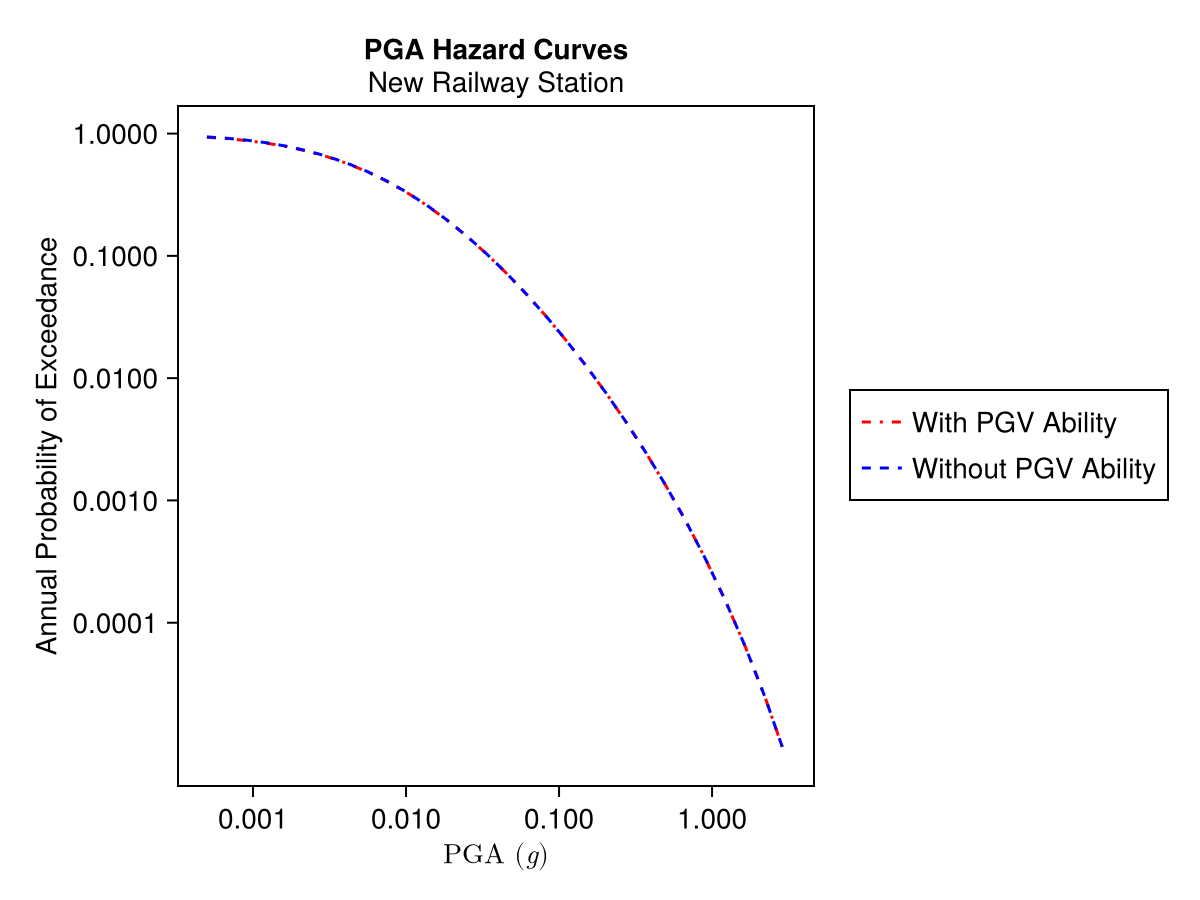
\includegraphics[width=\linewidth]{figures/hazard/logic_tree_comparison.png}
	\caption{Επιρροή Φαινομένων Τεκτονικών Πλακών}
	\label{fig:ltc}
\end{figure}

Στο Σχήμα \ref{fig:ltc} φαίνεται η σύγκριση της καμπύλης επικινδυνότητας στην θέση του Νέου Σιδηροδρομικού Σταθμού συμπεριλαμβάνοντας τις τεκτονικές πηγές, και αγνοώντας τις. Οι δύο καμπύλες ταυτίζονται, και επομένως οι συγκεκριμένες πηγές αγνοούνται, θεωρώντας ότι δεν μειώνεται η ακρίβεια των υπολογισμών. Δεδομένου ότι η Θεσσαλονίκη δεν βρίσκεται κοντά σε τεκτονικά ρήγματα (εκτός ίσως από της Βόρειας Ανατολίας στο Αιγαίο), είναι λογικό και η επιρροή αυτών να είναι μικρή, όπως είναι και των ηφαιστειακών πηγών. 

%EFEHR

% G-R MFD
Η μοντελοποίηση των πηγών σε πιθανοτικές αναλύσεις επικινδυνότητας, γίνεται φυσικά με κάποια κατανομή μεγέθους-συχνότητας (Magnitude Frequency Distribution, MFD). Η κατασκευή της κατανομής, γίνεται σύμφωνα με κάποια σχέση που ορίζει την πιθανότητα υπέρβασης ενός σεισμικού μεγέθους, μία σύνηθης περίπτωση είναι η Εξίσωση \ref{eq:GR} των Gutenberg και Richter.

Οι MFDs όμως, αποσκοπούν στον υπολογισμό της πιθανότητας εμφάνισης ενός συγκεκριμένου μεγέθους, και όχι ενός εύρους μεγεθών. Για να κατασκευαστεί μία τέτοια κατανομή, επιλέγεται πρώτα ένα πλάτος τμήματος (bin width), το οποίο συνήθως είναι ίσο με $0.1$, και υπολογίζεται η πιθανότητα εμφάνισης σεισμού, με μέγεθος εντός εύρους του τμήματος.

Δεδομένου ότι κάθε τμήμα έχει ένα ελάχιστο και ένα μέγιστο μέγεθος $M_{min}$ και $M_{max} = M_{min} + bw$ αντίστοιχα, όπου $bw$ το πλάτος του κάθε τμήματος, ο αριθμός εμφάνισης σεισμών στο τμήμα είναι ίσος με την διαφορά του αριθμού σεισμών που ξεπερνούν την τιμή $M_{min}$ με αυτών που ξεπερνούν την τιμή $M_{max}$.

Ο υπολογισμός αυτός μπορεί να περιγραφεί από την Εξίσωση \ref{eq:MFD}.

\begin{equation}
	N_b = 10^{(a - bM_{min})} - 10^{(a - bM_{max})}
	\label{eq:MFD}
\end{equation}

\begin{figure}
	\centering
	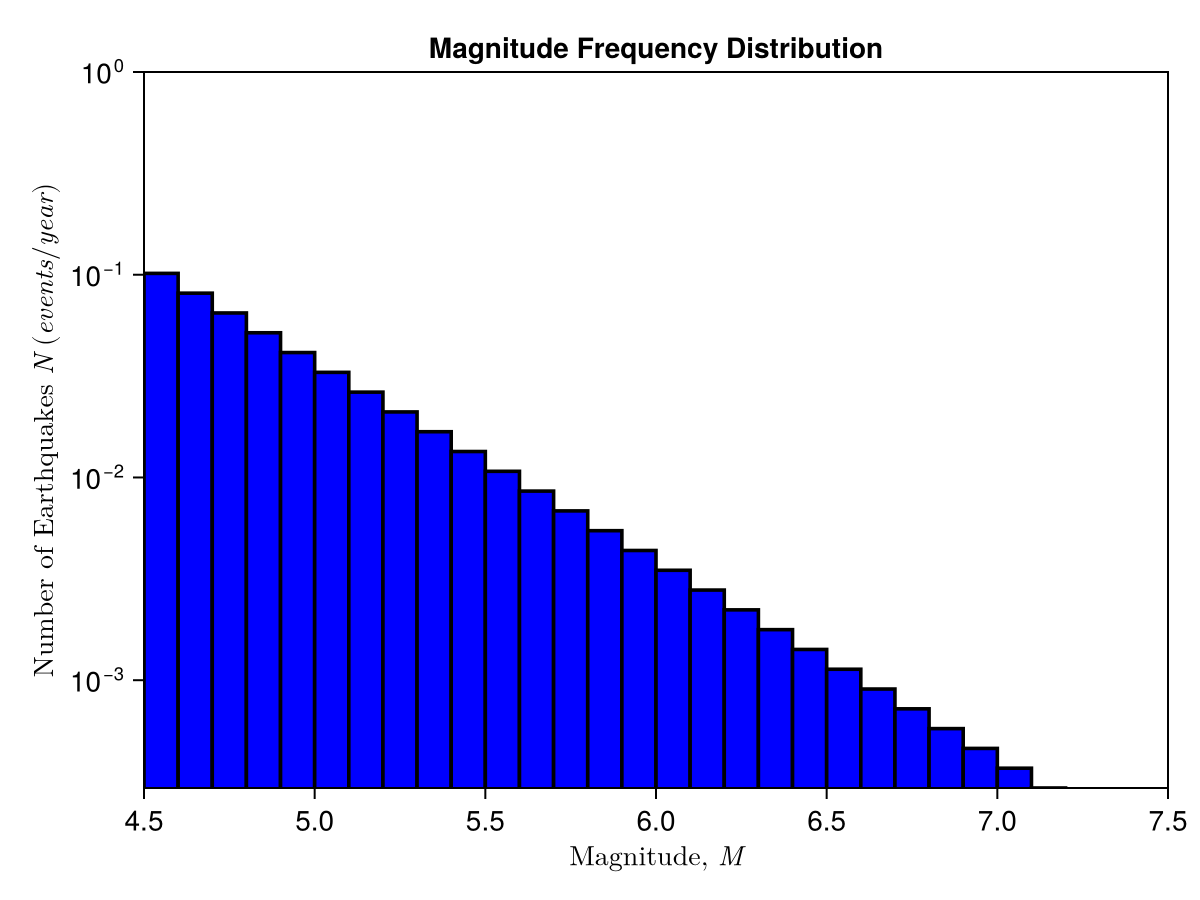
\includegraphics[width=\linewidth]{figures/hazard/MFD.png}
	\caption{Παράδειγμα Κατανομής MFD σε Χρησιμοποιούμενη Σεισμική Πηγή}
	\label{fig:MFD}
\end{figure}

Ακόμα, συχνά χρησιμοποιείται η αποκομμένη σχέση των Gutenberg-Richter, όπου ορίζεται ένα μέγιστο και ένα ελάχιστο μέγεθος $\bar{M}$ και $M_0$ αντίστοιχα, πέραν των οποίων ορίων η πηγή δεν μπορεί να δώσει σεισμούς.

Στο Σχήμα \ref{fig:MFD} απεικονίζεται ένα παράδειγμα μέσα από τις χρησιμοποιούμενες πηγές, η οποία προσομοιώνεται με αποκομμένη σχέση Gutenberg-Richter με παραμέτρους $a=4.0961$, $b=0.9673$, $M_0=4.5$ και $\bar{M}=7.2$.



\subsection{Εξασθένιση \& Πρόβλεψη Εδαφικής Κίνησης}
Η ισχυρή εδαφική κίνηση μπορεί να εκτιμηθεί με μία γενική σχέση όπως η Εξίσωση \ref{eq:GMPE} \parencite{Atik}. Τα μέλη που την συντελούν είναι ο φυσικός λογάριθμος ενός μεγέθους απόκρισης $Y$, η σχέση εξασθένισης $f(X_{es,\theta})$, το διάνυσμα μη-δεσμευμένων παραμέτρων $X_{es}$, οι συντελεστές του διανύσματος $\theta$ και μία τυχαία μεταβλητή που περιγράφει την μεταβλητότητα της κίνησης.

\begin{equation}
	Y = f(X_{es},\theta) + \Delta
	\label{eq:GMPE}
\end{equation}

Οι παράμετροι που επηρεάζουν την σχέση πρέπει να είναι αδέσμευτες έτσι ώστε η επιρροή κάθε ξεχωριστής παραμέτρου να συνεισφέρει ανεξάρτητα στην τελική κίνηση. Οι συνηθέστερες που χρησιμοποιούνται για τον ορισμό της σχέσης εξασθένισης είναι το μέγεθος ροπής $M_w$ και η απόσταση της θέσης από την πηγή. Οι αποστάσεις φέρουν πολλους τύπους αναλόγως, κυρίως, με την γεωγραφική σχέση πηγής-θέσης και μπορεί να είναι υποκεντρική, υποκεντρική, Joyner-Boore και άλλοι τύποι απόστασης.

Το μέγεθος και η απόσταση είναι οι βασικότεροι παράμετροι που χρησιμοποιούνται, αλλά έπειτα υπάρχουν παράμετροι για τον προσανατολισμό της πηγής, που μπορεί να δίνει έντονη εξασθένιση, τον τύπο της διάρρηξης και άλλων.

Σε σχέση με την περίπτωση της Θεσσαλονίκης, εφόσον οι κύριες πηγές που επηρεάζουν το έργο είναι επιφανειακές, έτσι και τα φαινόμενα που επικρατούν θα είναι φαινόμενα εγγούς πεδίου. Για αυτόν τον λόγο επιλέγονται κατάλληλες εξισώσεις, που να εκφράζουν σωστά τα επιφανειακά ρήγματα και να υπολογίζονται με χρήση τιμών $V_{s30}$ οι οποίες και είνα διαθέσιμες στο έργο όπου και χρησιμοποιήθηκαν σχέσεις κατά \cite{Kotha, Kotha2}.

%Δένδρο

Για να υπολογιστεί όμως η τελική ισχυρή εδαφική κίνηση, χρειάζεται να συνυπολογιστεί η συνεισφορά των τοπικών εδαφικών συνθηκών.

\subsection{Θέσεις Μελέτης}
\label{sbs:site}
Όπως αναφέρθηκε και στην Ενότητα \ref{Ch:intro}, η έκταση μελέτης αφορά στην γραμμή 1 του μετρό Θεσσαλονίκης, επομένως και οι τοπικές εδαφικές συνθήκες είναι οι αντίστοιχες της Θεσσαλονίκης.

Για την συνεκτίμηση των τοπικών εδαφικών συνθηκών, χρησιμοποιήθηκε η μέση ταχύτητα μετάδοσης διατμητικών κυμάτων $V_{s30}$ κατά μήκος των σηράγγων.

\begin{figure}[h]
	\centering
	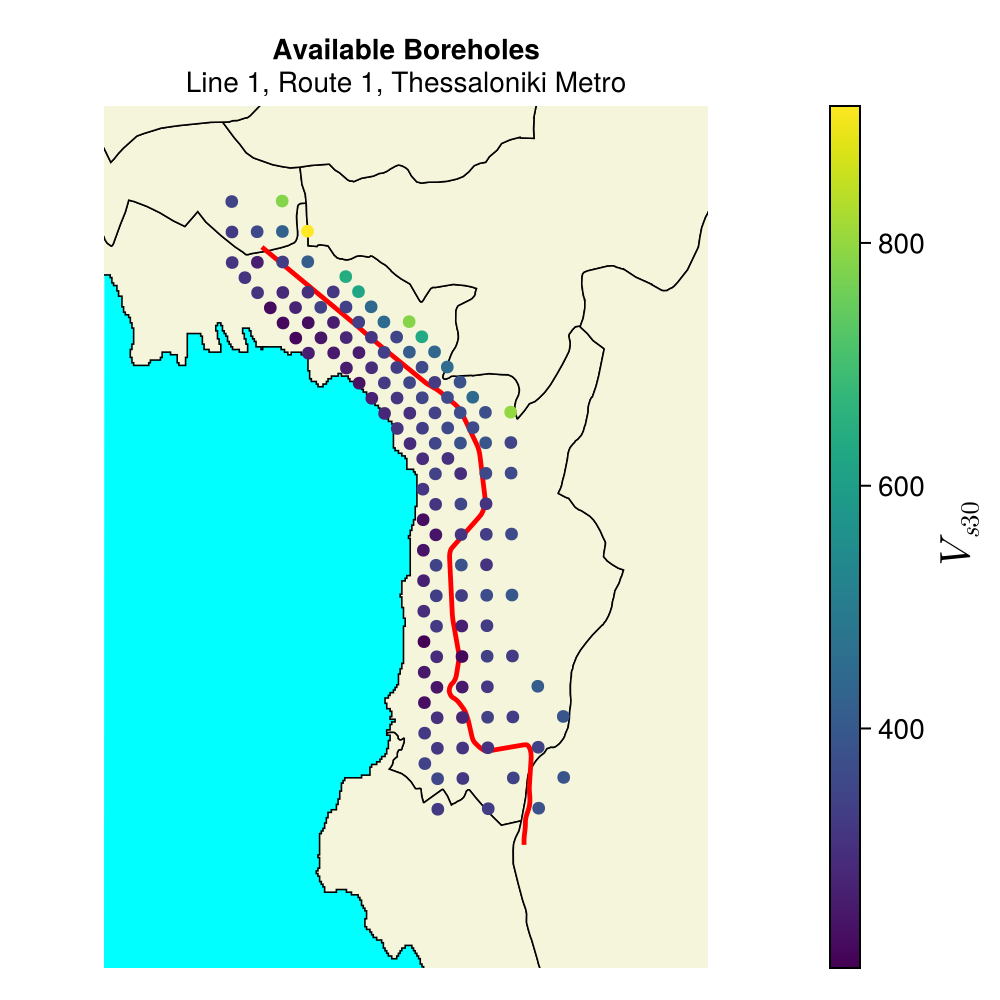
\includegraphics[width=0.95\linewidth]{figures/hazard/boreholes.png}
	\caption{Χρησιμοποιούμενες Γεωτρήσεις}
	\label{fig:bores}
\end{figure}

Η τιμή αυτή εκτιμήθηκε από μετρηθείσες τιμές σε διαθέσιμες γεωτρήσεις στον δήμο Θεσσαλονίκης και περιφερειακούς δήμους (βλ. Σχήμα \ref{fig:bores}), παρεμβάλοντας χωρικώς με χρήση της γεωστατιστικής μεθόδου Kriging \parencite{Krige}. Η μέθοδος Kriging χρησιμοποιεί διακυμανσογραφήματα πληθυσμού, για την εκτίμηση τιμών σε γεωγραφικές θέσεις που δεν έχουν διαθέσιμες μετρήσεις. Το πλεονέκτημα χρήσης της συγκεκριμένης μεθόδου, σε αντίθεση για παράδειγμα με γραμμική ή πολυωνμική παρεμβολή, είναι το γεγονός ότι συμπεριλαμβάνεται η έννοια της απόστασης στον υπολογισμό, σταθμίζοντας την βαρύτητα μίας θέσης μέτρησης με την εγγύτητα αυτής στην θέση εκτίμησης. Έτσι, δημιουργείται μία ομαλότερη παρεμβολή στον χώρο, και, αναλόγως με το μοντέλο και το φυσικό πρόβλημα, μια ακριβέστερη εκτίμηση. 

Στην συγκεκριμένη περίπτωση, χρησιμοποιείται κανονική διακυμανσιογράφημα ως η πιο απλή επιλογή, καθώς θεωρήθηκε ότι δεν απαιτείται κάτι πιο σύνθετο, ενώ τα σημεία δειγματοληψίας είναι αρκετά πυκνά για να θεωρηθεί ακριβής η μέθοδος.

Στο Σχήμα \ref{fig:map_m_vs} φαίνονται τα αποτελέσματα της παρεμβολής αποτυπωμένα σε χάρτη. Είναι σαφές ότι ενώ η παρεμβολή είναι επαρκώς ακριβής για την σήραγγα, η αποτύπωση στον χάρτη δίνει μία μάλλον ποιοτική παρά ορθολογική προσέγγιση του χώρου, αφού οι γεωτρήσεις που χρησιμοποιήθηκαν είναι όλες προς το μέσον του χάρτη, και γνωρίζοντας απομακρυνόμενος από την θάλασσα, κάποιος παρατηρητής θα συναντούσε την Άνω Πόλη, στην οποία επικρατούν κατά βάση βραχώδη επιφανειακές στρώσεις, και επομένως υψηλότερες τιμές $V_{s30}$. Αυτό αποτυπώνεται εν μέρη από τις λίγες υψηλές τιμές που βρίσκονται μακρύτερα από το θαλάσσιο μέτωπο.


\begin{figure}[h]
	\centering
	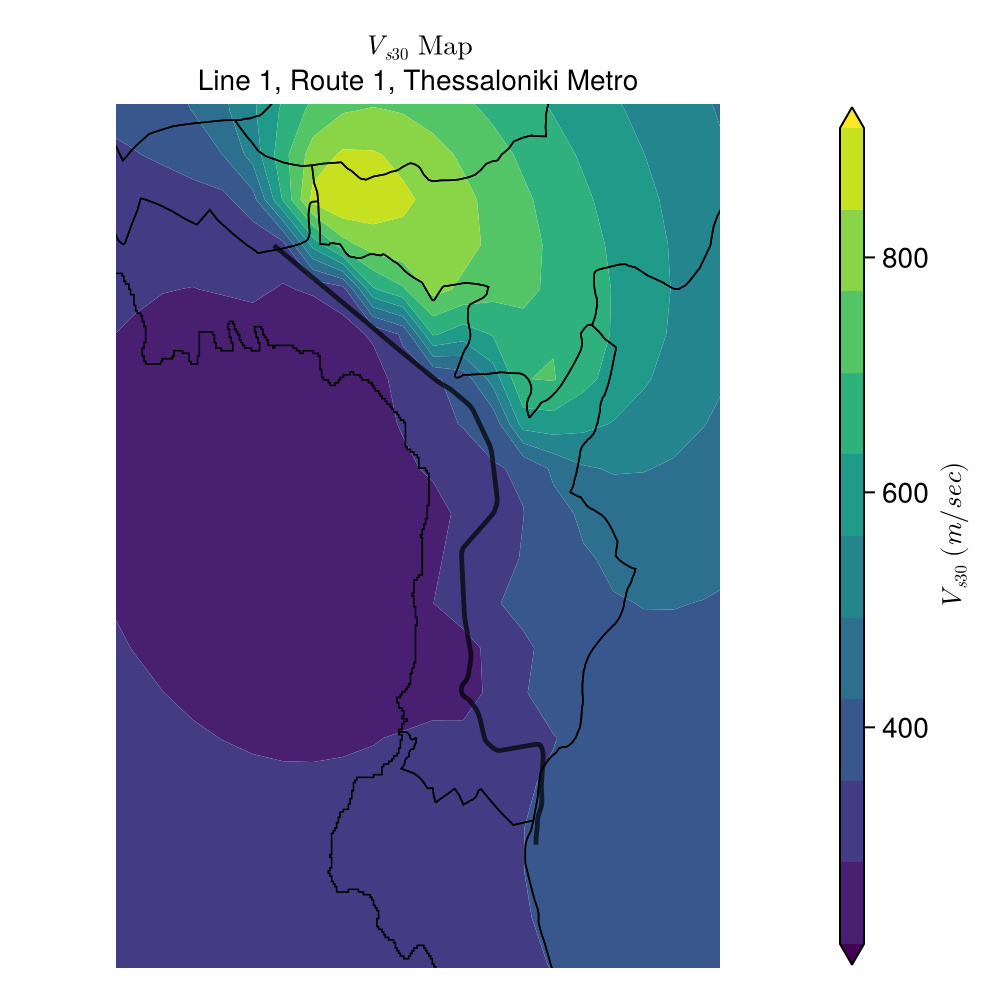
\includegraphics[width=0.95\linewidth]{figures/hazard/Map_measured_vs.png}
	\caption{Χάρτης τιμών $V_{s30}$ (Τιμές Γεωτρήσεων)}
	\label{fig:map_m_vs}
\end{figure}

Πέρα από τις τιμές των γεωτρήσεων, χρησιμοποιήθηκαν και άλλες τιμές για πλήθυνση και σύγκριση των αποτελεσμάτων. Εξού και χρησιμοποίηθηκαν τιμές από το European Seismic Risk Model \parencite{ESRM20}, το οποίο είναι ένα σύγχρονο εγχείρημα για καταγραφή της σεισμικής διακινδύνευσης στην Ευρώπη.

Το συγκεκριμένο μοντέλο έχει την Ευρώπη χωρισμένη σε ξεχωριστές τετραγωνικές γεωγραφικές υπόενότητες, ενός συγκεκριμένου γεωγραφικού πλάτους, όπου η κάθε μία έχει προϋπολογισμένες κάποιες τιμές παραμέτρων, όπως είναι η $V_{s30}$. Το μοντέλο δεν αποσκοπεί στην απόλυτη αναπαράσταση των πραγματικών συνθηκών, αλλά σε μία εποπτική εκτίμηση της διακινδύνευσης και είναι πολύ χρήσιμο για αναλύσεις σε μεγάλη γεωγραφική έκταση.


\begin{figure}[h]
	\centering
	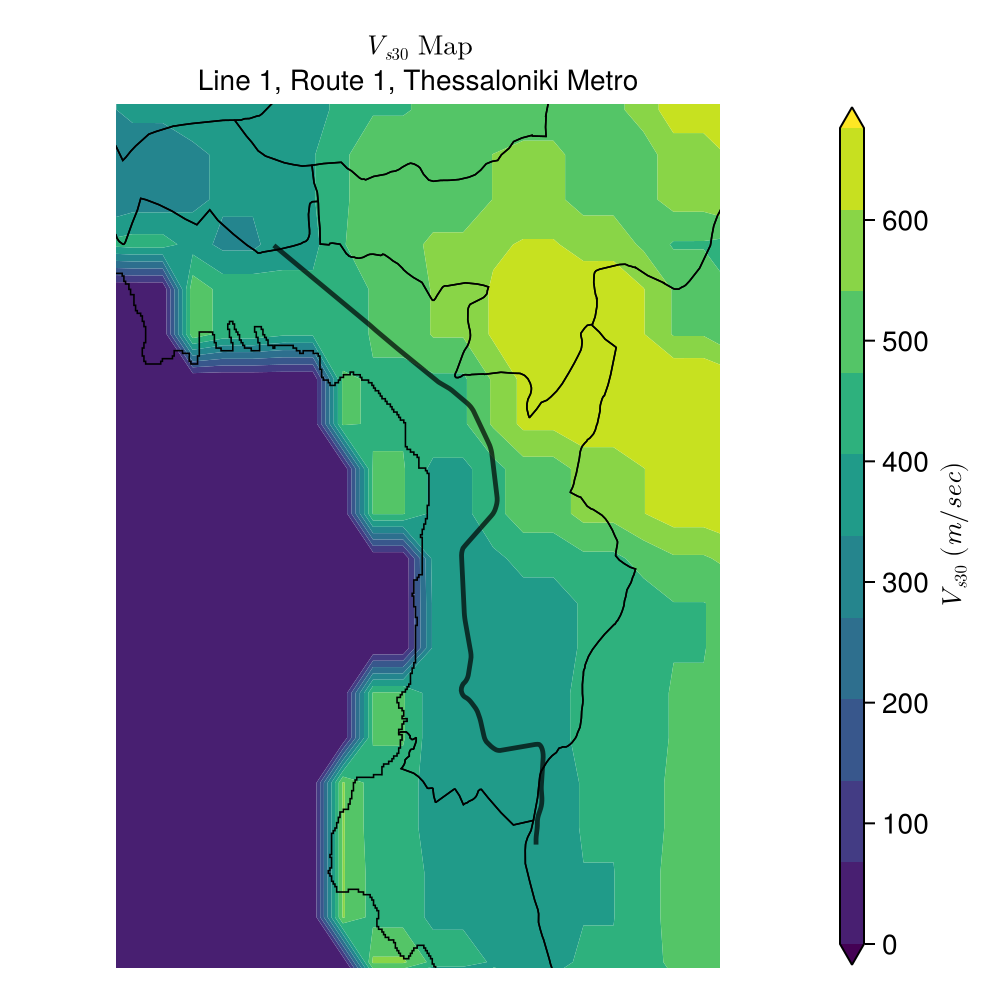
\includegraphics[width=0.95\linewidth]{figures/hazard/Map_assigned_vs.png}
	\caption{Χάρτης τιμών $V_{s30}$ (ESRM20 Sitemodel)}
	\label{fig:map_a_vs}
\end{figure}

Στο Σχήμα \ref{fig:map_a_vs} απεικονίζονται οι τιμές $V_{s30}$ για την υπό μελέτη περιοχή, όπως υπάρχουν στο ESRM20. Εδώ αναπαριστάται καλύτερα η κατανομή των εδφικών στρώσεων, με το βραχώδες υπόβαθρο να εμφανίζει τιμές περί τα $800\;m/sec$ (Κατηγορία Α) στην περιοχή που βρίσκεται η Άνω Πόλη και τις τιμές κοντά στην παραλία να έχουν χαμηλότερης κατηγορίας εδάφη B και C κατά τον Ευρωκώδικα 8.

Συγκρίνοντας τους δύο χάρτες κατά μήκος της σήραγγας, διαπιστώνεται ότι οι τιμές των γεωτρήσεων κυμαίνονται μεταξύ των $300-400\;m/sec$ ενώ οι τιμές του ESRM20 μεταξύ των $400-500\;m/sec$. Έτσι, όπως θα φανεί και στην συνέχεια, οι τιμές των γεωτρήσεων φαίνεται να είναι πιο συντηρητικές.

Αντίστοιχα, το OpenQuake διαθέτει έναν ακόμα τρόπο υπολογισμού της επικινδυνότητας, σύμφωνα με την τοπογραφική κλίση και την γεωλογία των επιφανειακών στρώσεων και όχι το $V_{s30}$. Αυτές οι παράμετροι προκύπτουν με τον ίδιο τρόπο από το ESRM20 και τα αποτελέσματα τους φαίνονται στην Ενότητα \ref{sc:hanal}. Η χρήση της γεωλογίας δεν χαρακτηρίζεται το ίδιο εύκολα όπως και με την $V_{s30}$, που είναι μία ευρέως χρησιμοποιούμενη τιμή, αλλά είναι επιθυμητό να γίνουν οι μέγιστες δυνατές συγκρίσεις στα αποτελέσματα της επικινδυνότητας.

\subsection{Λογικά Δένδρα}
\label{sbs:tree}
%Εδώ θα μπουν μερικά πολύ ωραία πράγματα για τα δέντρα και για την μότνεκαρλο. Τώρα θα γράψω από ένστικτο, αφού έκανα τα σχήματα , και παιστεύω ότι είναι αρκετά για τώρα, και θα πάω να κοιμηθώ που γράφω με κλειστά μάτια εξάλλλου. Άρα δεν ξέρω ακριβώς τι γράφω, το καώ που-καιπου σε τέτοιες καταστάσεις ( πολύ βέβαιος ότι εκεί έχει ένα μηδέν). Τώρα, άρα, τα δέντρα είναι τρόπος για υπολογισμός, δεν έχειε νόημα να έχουμε μόνο μία περίπτωση, βασικά στην πιθανοτική, ακριβώς, έχει νόημα να έχουμε περισσότερες, καια άρα τις βάζουμε στα δέντρα. Το βασικό πλεονέκτημα είναι ότι μπορούν να έχουν πολλές μαζί και να σταθμίζονται κατάλληληα, δίνει έτσι μία ακριβή και ολιστική προσέγγιση στο ζήτημα και είναι πολύ καλό τρ δέντρο γενικά. Το κακό είναι ότι πρέπει να έχεις έναν εξπέρτ να σου τα κατασκευάσει και υπάρχει πολύ υποκειμενικότητα στις επιλογές αυτές. Επίσης το πως γίνεται, βγαίνουν οι κλάδοι και τετοια, γινόμενα και μπλα-μπλα. Κάποιες φορές οι κλάδοι μπορεί να είναι ´τοσοι πολλοί που δεν γίνεται και κάνουμε μόντε κάρλο που είναι αυτ'ο που είναι και θα περιγράψω. Επίσης να πω μετά για την δική μου περίπτωση, πολλά πράγματα άλλα δύσκολ υπολογιστικά να βάλουμε full enumeration και έτσι έχουμε μόντε κάρλο, βέλτιστος αριθμός δειγμάτων; τον βρήκαμε υπολογιστικά και αυότ είναι αυτό, βάζουμε και τα ´αλλα δύο σχήματα εδώ και είμαστε συγκεντρωμένοι. μετά θα πάω στις αναλύσεις και τα αποτελέσματα τους. Ίσως πρέπει να αλλάξω τον τίτλο της ενότητας σε Αποτελέσματα Αναλύσεων αντί για αναλύσεις, γιατί έχω γράψει ήδη πολλά για αναλύσεις εκτός. Δεν έγραψα και τόσες πολλές λέξεις, βέβαια δεν έχω και παραγράφους για να χωρέσουν. Τέλος πάντων, δέκα λεπτά κάθισα για να τα γράψω όλα κι όλα.

Ο υπολογισμός της σεισμικής επικινδυνότητας, μπορεί να γίνει μεμονομένα για μία συγκεκριμένη πηγή, με κάποια σχέση εξασθένισης και γνωρίζοντας τις τοπικές εδαφικές συνθήκες, όλα με δοσμένες παραμέτρους. Η πιθανοτική μέθοδος όμως, δεν αποσκοπεί στον υπολογισμό ενός χαρακτηριστικού σεισμού όσο σε μία στατιστική πρόβλεψη της πιθανότητας εμφάνισης κάθε σεισμικού γεγονότος.

Η εκτίμηση της υψηλότερης επικινδυνότητας για πλήθος πηγών και σχέσεων εξασθένισης και ισχυρής εδαφικής κίνησης είναι ένα σύνθετο πρόβλημα, για αυτό και τα λογικά δένδρα χρησιμοποιούνται για τον υπολογισμό της σταθμισμένης πιθανότητας.

Πριν από την κατασκευή του, ένα λογικό δένδρο μπορεί να περιγραφεί μαθηματικά όπως και στην Εξίσωση \ref{eq:tree}, όπου $v_n(z|\theta_n)$ πρόκειται για την πιθανότητα εμφάνισης της εδαφικής κίνησης $z$ για δεδομένες παραμέτρους $\theta_n$. Η πιθανότητα αυτή εκφράζεται ως το άρθοισα των γινομένων των τριών πιθανοτήτων $\lambda_n(M_i|\theta_n$,  $P_n(r_j|M_i,\,\theta_n)$ και $G(z|M_i,\,r_j,\,\theta_n)$ όπου είναι η πιθανότητα να εμφανιστούν σεισμός που ξεπερνάει μέγεθος $M_i$, η κρίσιμη απόσταση θέσης-πηγής να είναι $r_j$ και η πιθανότητα η ένταση να ξεπερνάει ένταση $z$ δεδομένου πάντα ορισμένων παραμέτρων. \parencite{Kulkarni}

\begin{equation}
	v_n(z|\theta_n) = \sum_i\sum_j \lambda_n(M_i|\theta_n)\cdot P_n(r_j|M_i,\,\theta_n)\cdot G(z|M_i,\,r_j,\,\theta_n)
	\label{eq:tree}
\end{equation}

Το άθροισμα αυτών των γινομένων, κατασκευάζει προφανώς ένα λογικό δέντρο. Σκοπός του εξάλλου είναι η χαρτογράφηση κάθε δυνατής εδαφικής κίνησης, όπου συνυπολογίζοντας τα βάρυ αυτών προκύπτει η συνολική πιθανότητα.

\begin{figure}
	\centering
	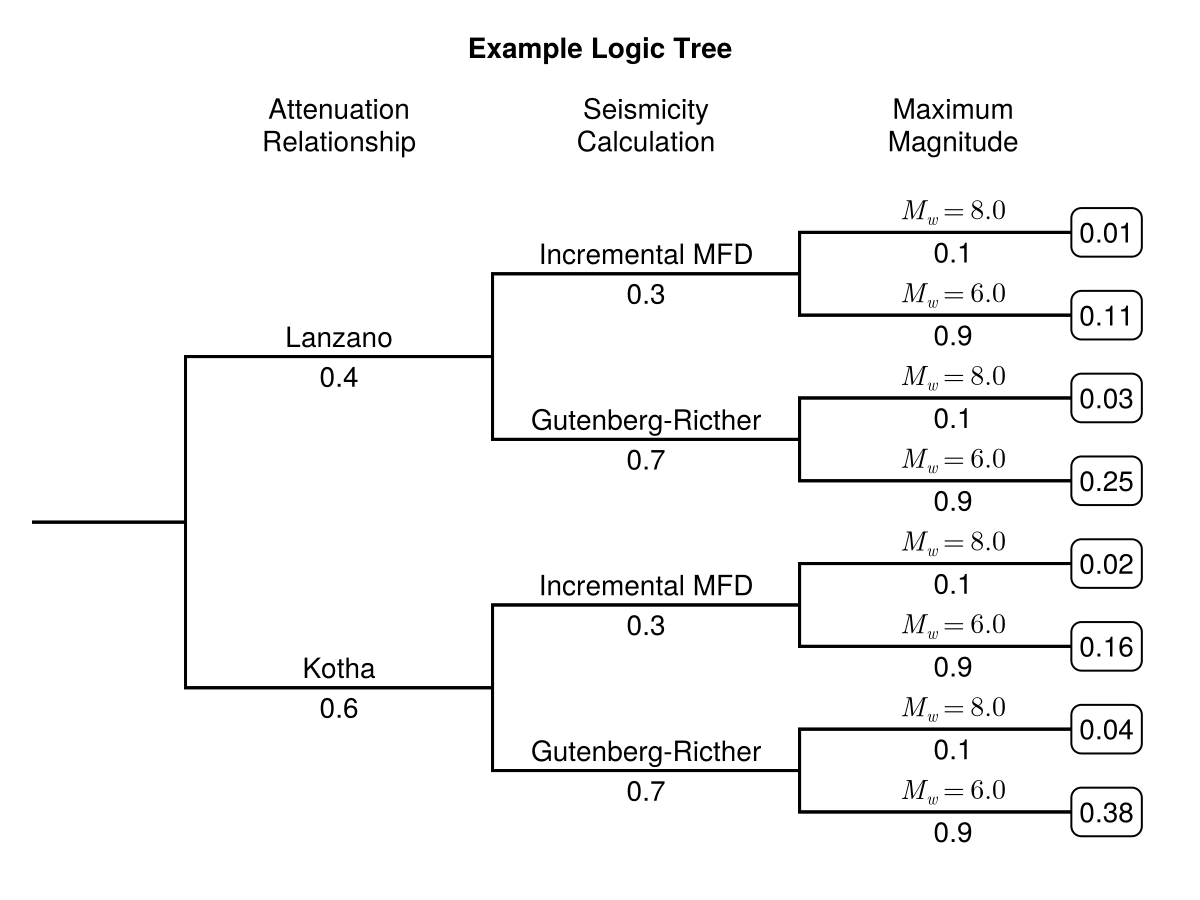
\includegraphics[width=0.95\linewidth]{figures/hazard/tree.png}
	\caption{Παράδειγμα Λογικού Δέντρου}
	\label{fig:tree}
	
\end{figure}

Ένα περιορισμένο παράδειγμα εμφανίζεται στο Σχήμα \ref{fig:tree}, όπου το δένδρο έχει μόνο τρία επίπεδα. Σε πραγματικές περιπτώσεις, οι παράμετροι δύναται να είναι αρκετοί, και να παίρνουν πολλές τιμές δηιουργώντας ένα δένδρο με χιλιάδες κλάδους, δυσκολεύοντας τον υπολογισμό.

Επομένως, δεν είναι πάντα υπολογιστικώς συμφέρον να εκτελεστεί η πλήρης ανάλυση για κάθε περίπτωση. Σε αυτή την περίπτωση, το OpenQuake χρησιμοποιεί την μέθοδο Monte Carlo για στατιστική προσέγγιση της ακριβούς λύσης.

Η μέθοδος Monte Carlo πρόκειται για μία στατιστική μέθοδος προσέγγισης φυσικών προβλημάτων, κατά την οποία λαμβάνεται ένα σύνολο από τυχαία δείγματα που ερμηνεύονται από κάποια στατιστική κατανομή προσεγγίζοντας έτσι μία διαφορική εξίσωση συνήθως με διακριτές τιμές \parencite{Metropolis}.

Στην συγκεκριμένη περίπτωση, τα δείγματα της Monte Carlo σε ένα λογικό δένδρο λαμβάνονται επιλέγοντας κάθε φορά από έναν διαφορετικό κλάδο και συγκρατώντας το αποτέλεσμα. Ο τρόπος που επιλέγονται οι κλάδοι είναι πολύ απλός, πρώτα κατασκευάζεται μία συνάρτηση κατανομής για κάθε δένδρο όπως φαίνεται στο Σχήμα \ref{fig:MonteCarlo}, έπειτα κάθε δείγμα παράγει μία ξεχωριστή τιμή ανάμεσα σε εύρος [0, 1] η οποία αντιστοιχεί στον κλάδο που έχει την πρώτη συσσωρευτική τιμή που την ξεπερνάει. Για παράδειγμα, αν ένα δείγμα έχει τιμή 0.3, το συγκεκριμένο δείγμα θα αντιστοιχεί στον κλάδο B3.

\begin{figure}
	\centering
	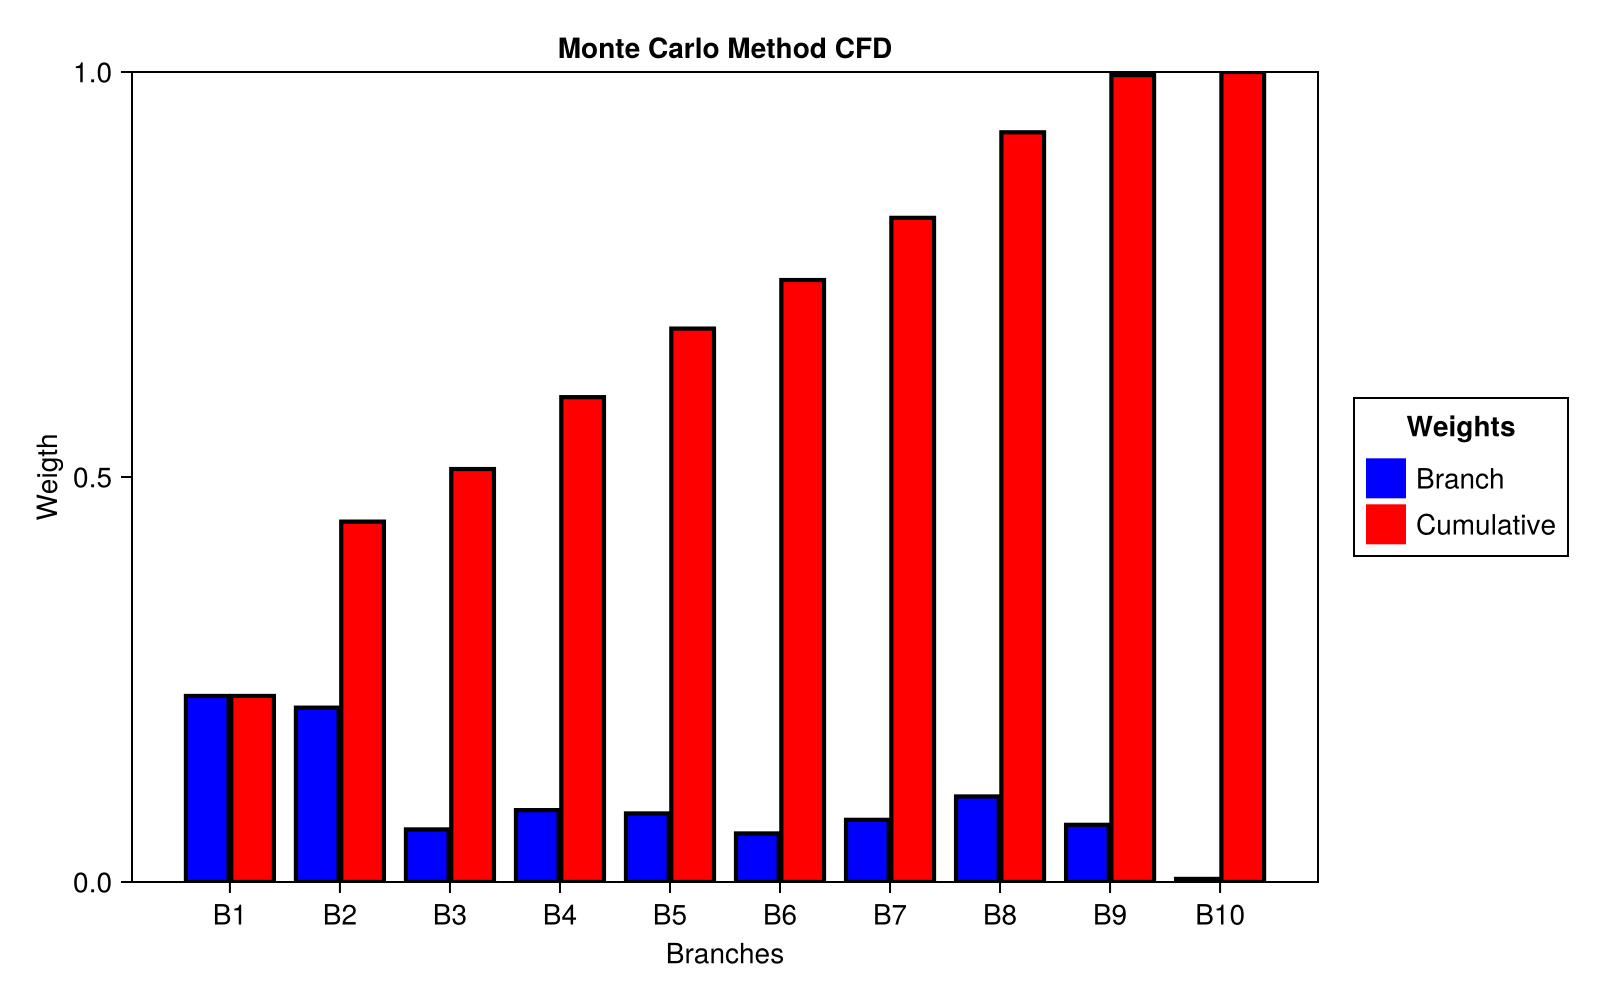
\includegraphics[width=\linewidth]{figures/hazard/monte-carlo.png}
	\caption{Παράδειγμα της Μεθόδου Monte Carlo}
	\label{fig:MonteCarlo}
\end{figure}

Είναι προφανές λοιπόν ότι η άθροιση αρκετών κλάδων θα πλησιάσει ικανοποιητικά την μοναδιαία τιμή ενώ σε περίπτωση που υπολογιστούν όλοι οι κλάδοι, τότε δεν πρόκειται για μέθοδο Monte Carlo αλλά για τον πλήρη υπολογισμός λογικού δένδρου (Full Enumeration).

Η "τύχη", στις τιμές των δειγμάτων, ορίζεται από κάποιον αλγόριθμο παραγωγής αριθμοσειρών και δεν είναι πραγματική τυχαιότητα για υπολογιστική οικονομία αλλά και για να είναι τα αποτελέσματα αναπαραγωγίσιμα.

Καθώς η ανάλυση επικινδυνότητας στο μετρό Θεσσαλονίκης αφορά πολλά σημεία, ο συνολικός όγκος αναλύσεων είναι αρκετά μεγάλος ώστε να προτιμηθεί η χρήση περιορισμένου αριθμού δειγμάτων αντί πλήρους υπολογισμού.

Ο αριθμός δειγμάτων επιλέχθηκε με βασικότερο κριτήριο την ακρίβεια αποτελεσμάτων, εποπτεύοντας ποιοτικά το σημέιο όπου η εκτιμώμενη επικινδυνότητα προσεγγίζει μία σταθερή τιμή, και θέτοντας τον αριθμό των δειγμάτων ίσο με αυτό το νούμερο.

\begin{figure}[h]
	\centering
	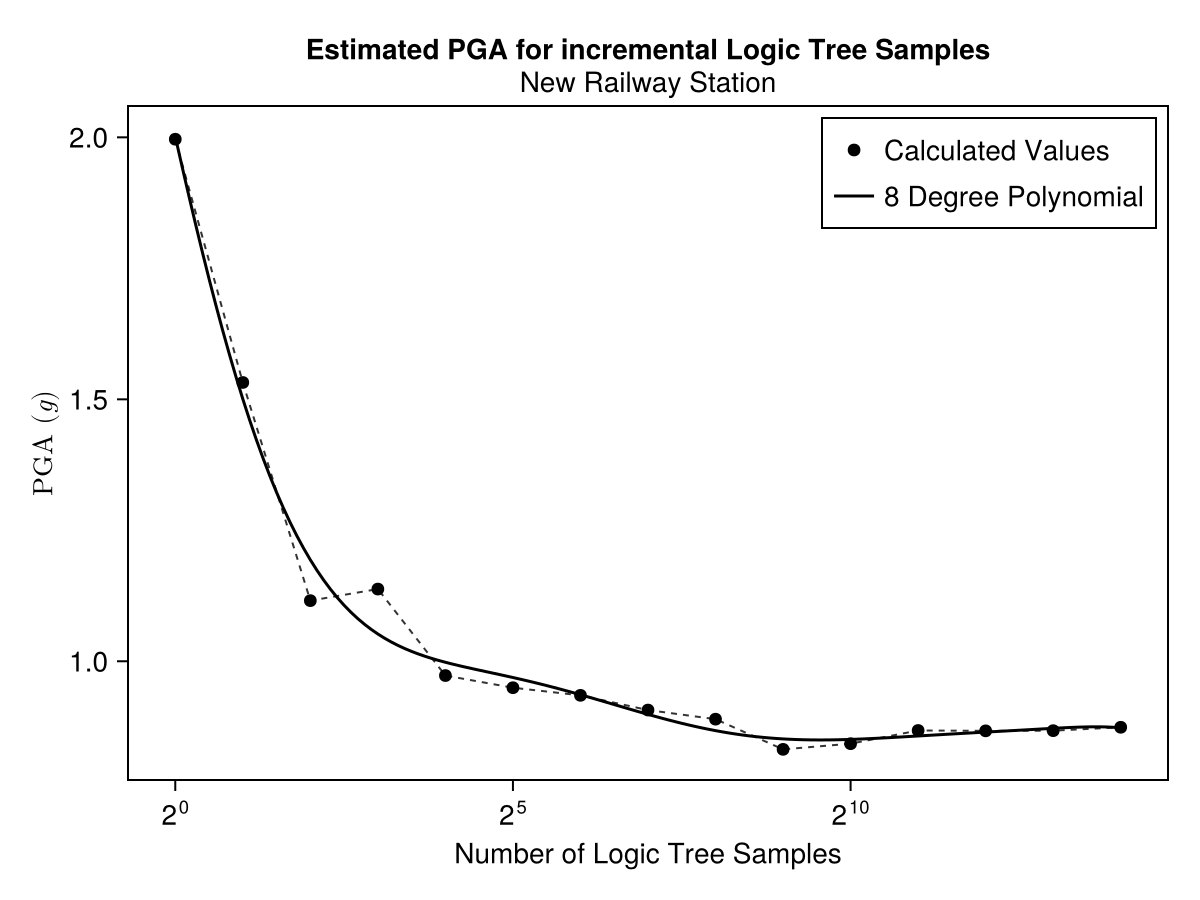
\includegraphics[width=0.9\linewidth]{figures/hazard/core_number.png}
	\caption{Εύρεση Βέλτιστου Αριθμού Δειγμάτων}
	\label{fig:cores}
\end{figure}

Η επιλογή αριθμού δειγμάτων έγινε με την πραγματοποίηση 15 ξεχωριστών αναλύσεων στην θέση του Νέου Σιδηροδρομικού Σταθμού και εκτιμώντας την PGA για περίοδο επαναφοράς 2500 έτη. Ο αριθμός δειγμάτων σε κάθε επανάληψη προέκυψε ως η εκθετική συνάρτηση $2^n$ με τιμές του $n$ από 0 έως 14.

Στο Σχήμα \ref{fig:cores} αποτυπώνονται τα αποτελέσματα των αναλύσεων με ένα πολυώνυμο ογδόου βαθμού να παρεμβάλεται στις τιμές. Από αυτά τα αποτελέσματα επιλέγεται τιμή για κάθε ανάλυση ίση με 1000 δείγματα καθώς μετά από αυτό το σημείο η επικινδυνότητα παρουσιάζει πολύ ελαφρά αύξηση, σε σχέση με πολύ μεγάλη αύξηση του αριθμού δειγμάτων.

Με μικρότερο αριθμό αναλύσεων, αποτυπώνονται στο Σχήμα \ref{fig:l_samples} κατά-μήκος αποτελέσματα για 1, 128 και 1024 δείγματα αντίστοιχα καθώς και καπμύλες επικινδυνότητας για τον Νέο Σιδηροδρομικό Σταθμό. Είναι σαφές, για ένα μεγαλύτερο αριθμό σημείων, ότι η πρώτη αύξηση του αριθμού δειγμάτων έχει πολύ μεγάλη μεταβολή στην εκτιμώμενη επικινδυνότητα, ενώ η περαιτέρω αύξηση μειώνει σημαντικά την επίδραση της.

\begin{figure}[h]
	\centering
	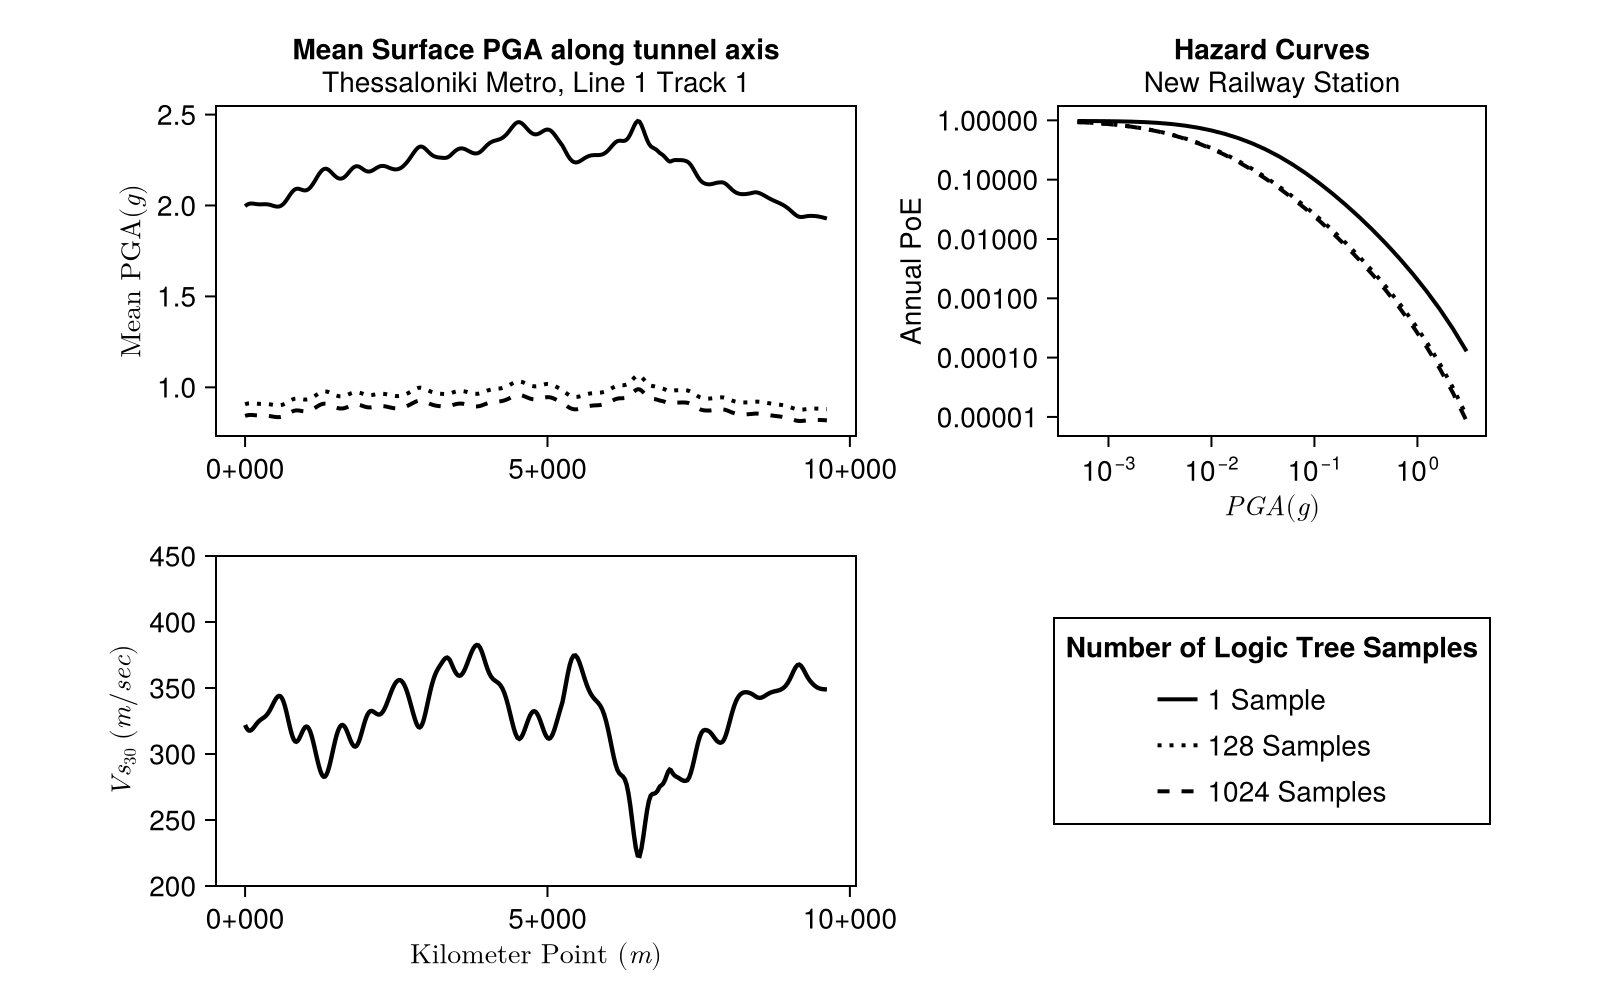
\includegraphics[width=1.\linewidth]{figures/hazard/longitudinal_samples.png}
	\caption{Σύγκριση Αποτελεσμάτων Αριθμού Δειγμάτων}
	\label{fig:l_samples}
\end{figure}

Έχοντας μελετήσει την χρήση των λογικών δένδρων, είναι απαραίτητο να αναφερθεί ότι η μεγαλύτερη δυσκολία στα δένδρα δεν είναι η χρήση αλλά η κατασκευή των, η οποία χρειάζεται να γίνεται από έμπειρους επιστήμονες. Η κατασκευή ενός λογικού δένδρου, απαιτεί μεγάλες γνώσεις τόσο στην γεωτεχνική σεισμική και σεισμολογία όσο και στις θέσεις που μελετόνται.

Τα λογικά δένδρα δίνουν μεγάλη ελευθερία στον ερευνητή, επιτρέποντας την μελέτη συγκεκριμένων θέσεων ή προβλημάτων εκτίμησης σεισμικής επικινδυνότητας, αλλά αυτή ακριβώς η ελευθερία είναι που επιφέρει την ευθύνη για την ακρίβεια των αποτελεσμάτων, πρώτα στον μελετητή και έπειτα στο υπολογιστικό εργαλείο.

% Εδώ πρέπει να βάλω λίγο κείμενο για την κατασκευή των λογικών δένδρων, πρέπει να ζητήσω παραπάνω πληροφορίες.

\section{Αποτελέσματα Αναλύσεων}
\label{sc:hanal}
% Η ενότητα των αναλύσεων μπορεί να είναι αχρείαστη και να είναι καλύτερα απλώς τα συμπεράσματα να είναι ξεχωριστή ενότητα, και τα των αναλύσεων να μπουν στις προηγούμενες υποενότητες

Έχοντας συγκεντρώσει και κατασκευάσει τις τα μοντέλα πηγών, τα λογικά δέντρα πρόβλεψης της ισχυρής εδαφικής κίνησης και οι θέσεις μελέτης, το επόμενο βήμα είναι η εκτέλεση των αναλύσεων που θα αποδώσουν την εκτιμηθείσα επικινδυνότητα. Τα αποτελέσματα αυτών παρατίθενται στην συγκεκριμένη ενότητα.

Τα αποτελέσματα που οι αναλύσεις παράγουν και ενδιαφέρουν στην μελέτη χωρίζονται σε δύο βασικές κατηγορίες. Στις τιμές εκτίμησης της σεισμικής επικινδυνότητας για συγκεκριμένη πιθανότητα εμφάνισης σεισμού σε ένα έτος, και σε καμπύλες επικινδυνότητας.

Οι τιμές της σεισμικής επικινδυνότητας αποτυπώνονται για συγκεκριμένες πιθανότητες εμφάνισης κατά μήκος της Τροχιάς 1 του μετρό Θεσσαλονίκης και σε χάρτη της πόλης της Θεσσαλονίκης. Οι καμπύλες επικινδυνότητας αποτυπώνονται σε τρεις χαρακτηριστικές θέσεις του μετρό.

\subsection{Διαμήκη Αποτελέσματα}
Τα βασικότερα αποτελέσματα που παράγονται από το OpenQuake είναι η εκτιμηθείσα επικινδυνότητα κατά μήκος του άξονα του μετρό. Τα αποτελέσματα που παρουσιάζονται είναι κατά μήκος της τροχιάς 1 στην πρώτη γραμμή του μετρό Θεσσαλονίκης, θεωρώντας ότι οι τιμές έιναι ίσες κατά μήκος των δύο τροχιών.

Πρώτα γίνεται μία σύγκριση μεταξύ των τριών μεθόδων επίλυσης που χρησιμοποιούνται, σύμφωνα με την προέλευση των δεδομένων. Στο Σχήμα \ref{fig:l_meth} απεικονίζονται τα αποτελέσματα της ανάλυσης.

Στο κάτω αριστερά υπό-σχήμα γίνεται η διαμήκης σύγκριση των τιμών $V_{s30}$ μεταξύ των γεωτρήσεων και των προβλέψεων ESRM. Οι γεωτρήσεις έχουν τυπικά χαμηλότερες τιμές, προδιαθέτοντας για συντηρητικότερες τιμές έντασης όπως αναφέρεται και στην Υποενότητα \ref{sbs:site}.

Στο πάνω-αριστερά υπό-σχήμα απεικονίζεται η εκτίμηση της σεισμικής επικινδυνότητας για περίοδο επαναφοράς 2500 ετών. Στο σχήμα επιβεβαιώνεται το γεγονός ότι οι τιμές των γεωτρήσεων προσφέρουν τις πλέον συντηρητικές τιμές. Οι τιμές για τις δύο μεθόδους κατά ESRM20 έχουν πολύ παρόμοιες τιμές, και υποεκτιμημένες σε σχέση με τις γεωτρήσεις.
	
Ακόμα, στο πάνω-δεξιά υπό-σχήμα σχεδιάζονται η καμπύλη επικινδυνότητας για κάθε μέθοδο στον Νέο Σιδηροδρομικό Σταθμό. Σε χαμηλές τιμές έντασης, η περίοδος επαναφοράς ταυτίζεται σχεδόν σε κάθε μέθοδο, ενώ τα πιο σπάνια ισοπιθανοτικά μεγέθη είναι μεγαλύτερα στις τιμές των γεωτρήσεων, γεγονός που γίνεται σαφές λόγω της λογαριθμικής κλίμακας του κάθε άξονα.

Από όλα τα ανωτέρω, προκύπτει ότι οι τιμές $V_{s30}$ που υπολογίστηκαν από τις γεωτρήσεις εκτιμούν τις κρισιμότερες τιμές επικινδυνότητας, επομένως, σε συνδυασμό με την προδιατεθημένη αξιοπιστία των δεδομένων, τα αποτελέσματα της συγκεκριμένης μεθόδου θα χρησιμοποιηθούν στην εκτίμηση της διακινδύνευσης.

Αφού συγκρίθηκαν οι τρεις μέθοδοι, και επιλέγη η πλέον κατάλληλη, υπολογίζεται η διαμήκης τιμή της έντασης για τις τρεις σημαντικές περιόδους επαναφοράς κατά τον αναθεωρημένο Ευρωκώδικα 8.

\begin{figure}[h]
	\centering
	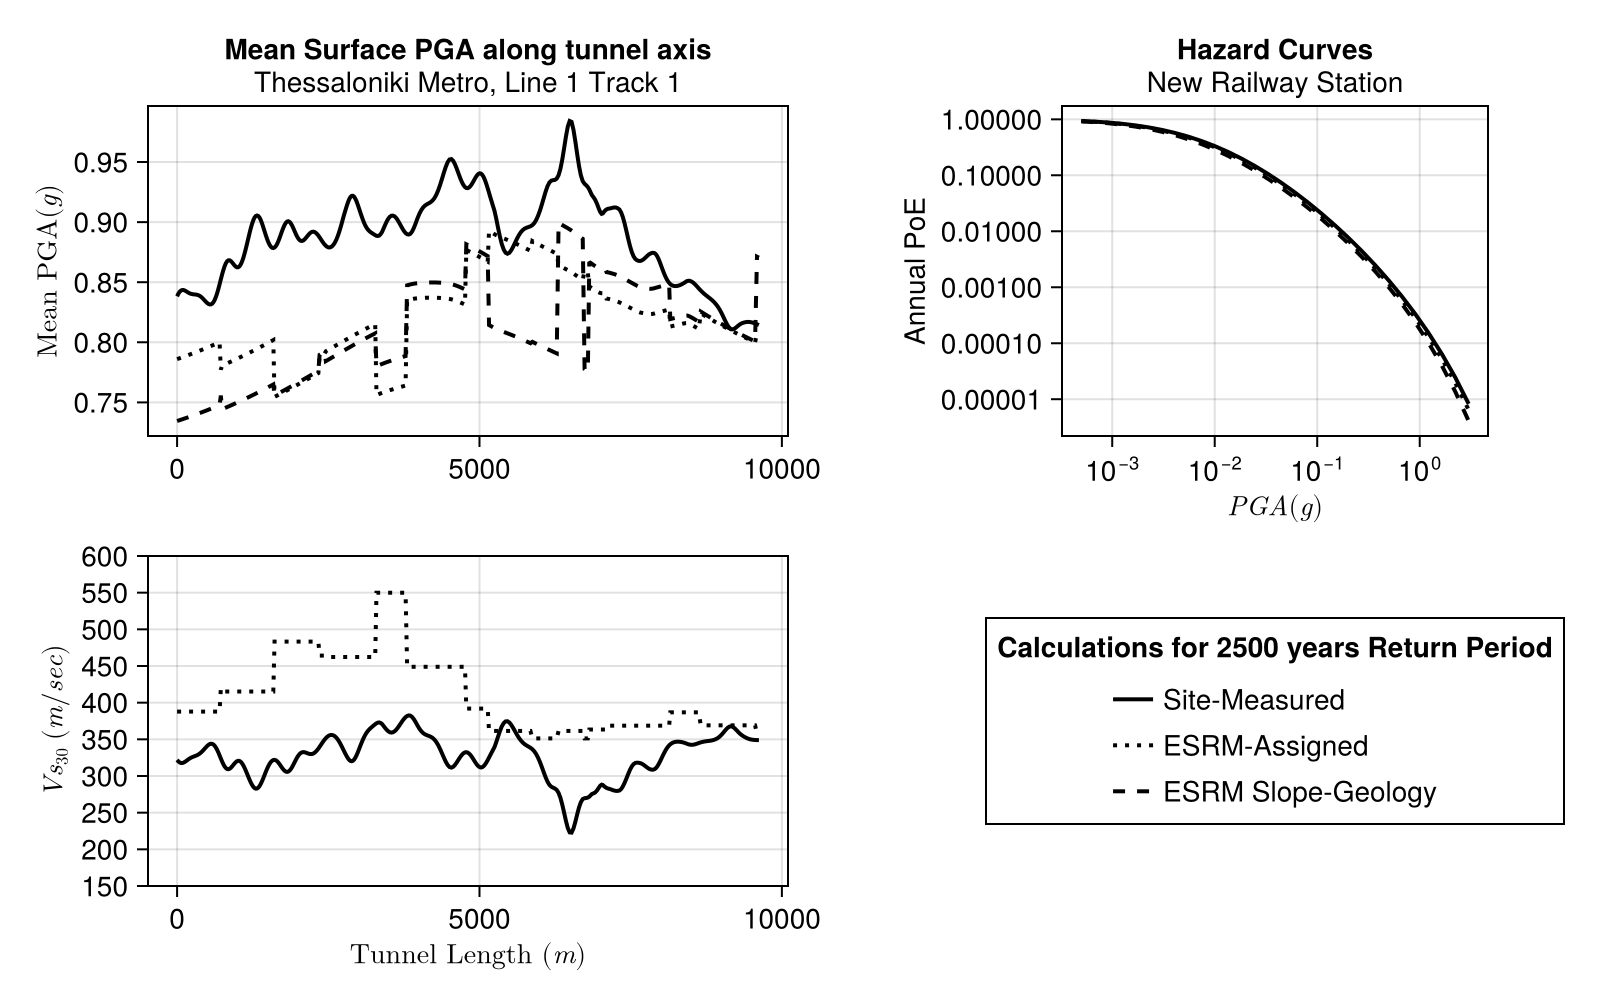
\includegraphics[width=\linewidth]{figures/hazard/method_comparison.png}
	\caption{Σύγκριση Μεθόδων}
	\label{fig:l_meth}
\end{figure}

Τα αποτελέσματα αποτυπώνονται στο Σχήμα \ref{fig:l_mean}. Προφανώς η αύξηση της περιόδου επαναφοράς αυξάνει την τιμή της επικινδυνότητας σε κάθε σημείο, ενώ ενδιαφέρον παρουσιάζει ότι η κάθε καμπύλη "μεγενθύνεται" σε μεγαλύτερες περιόδους, δηλαδή οι συχνότεροι σεισμοί έχουν μεγαλύτερη ομοιομορφία στον χώρο, ενώ τα ισχυρότερα σεισμικά γεγονότα διαφοροποιούνται σημαντικότερα στα ακρότατα των. Λογικά σε αυτό ευθύνεται η επιρροή που έχουν οι τοπικές εδαφικές συνθήκες, όπως φαίνεται από την σύγκριση των τιμών επικινδυνότητας με των $V_{s30}$, παρουσιάζοντας τοπικά ακρότατα σε παρόμοιες κατά βάση θέσεις.

\begin{figure}[h]
	\centering
	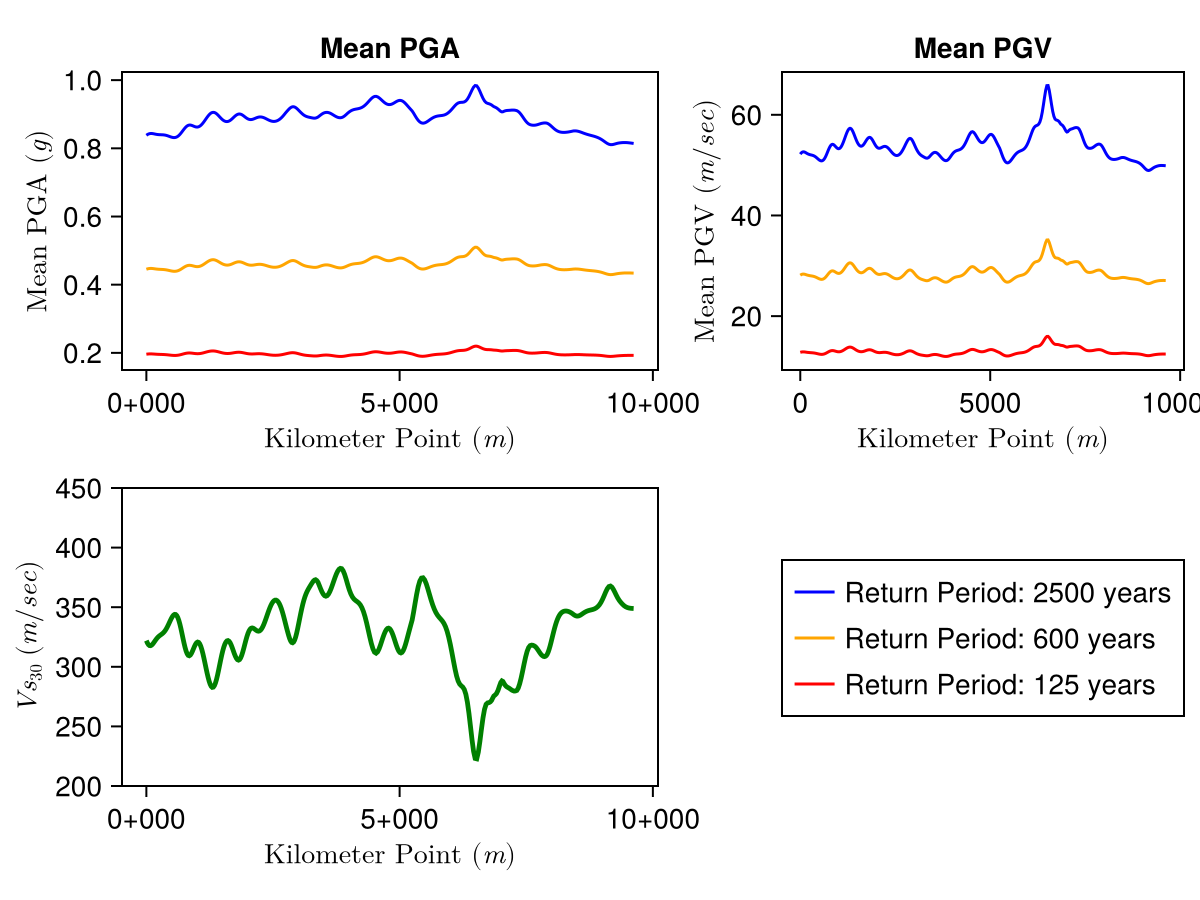
\includegraphics[width=\linewidth]{figures/hazard/long_pga-pgv.png}
	\caption{Μέσες Τιμές Έντασης Κατά Μήκος της Γραμμής}
	\label{fig:l_mean}
\end{figure}

Το παραγόμενο σχήμα προσφέρει μία πολύ σημαντική ποιοτική λεπτομέρεια, που είναι ότι η τάξη μεγέθους για τα μεγέθη έντασης είναι κατά μέσο $0.85g$ και $55\;cm/sec$ PGA και PGV αντίστοιχα για περίοδο επαναφοράς 2500 ετών.

\subsection{Καμπύλες Επικινδυνότητας}
Οι καμπύλες επικινδυνότητας (Hazard Curves) είναι ένας τρόπος απεικόνισης της επικινδυνότητας μίας θέσης. Πρόκειται για την συνάρτηση της πιθανότητας εμφάνισης ενός μεγέθους έντασης συναρτήσει του μεγέθους αυτού.

Όπως είναι προφανές, η πιθανότητα εμφάνισης ενός σεισμικού συμβάντος μειώνεται πάντα καθώς το μέγεθος του συμβάντος αυξάνεται. Έτσι οι καμπύλες επικινδυνότητας είναι γνησίως φθίνουσες συναρτήσεις. Αυτό είναι μία παραδοχή που έχει εμφανιστεί ήδη πολλές φορές στην συγκεκριμένη εργασία, όπου στην σεισμική μηχανική και αφορούν την παραγωγή σεισμών στις πηγές, όπως περιγράφεται για παράδειγμα από την Εξίσωση \ref{eq:GR} των Gutenberg-Richter. Δεδομένου ότι δεν έχει συμβεί κάποιος σεισμός και ότι η εκδήλωση ενός σεισμικού γεγονότος είναι άσχετη κάθε άλλου, τότε κάθε σεισμός έχει πιθανότητα εμφάνισης αντιστρόφως ανάλογης με το μέγεθος του.

Από μόνες τους οι καμπύλες περιγράφουν την κατανομή των σεισμικών συμβάντων, αλλά η χρησιμότητα τους διαφαίνεται καλύτερα στην παραγωγή καμπυλών διακινδύνευσης σε πιθανοτικές αναλύσεις εκτίμησης της διακινδύνευσης (Probabilistic Seismic Risk Assessment, PSRA).

Όπως θα αναπτυχθεί στο ερχόμενο κεφάλαιο, οι καμπύλες τρωτότητας αναπτύσσονται αποκλειστικά σε τρεις χιλιομετρικές θέσεις λόγω του υπολογιστικού κόστους που επιβάλλουν οι δυναμικές αριθμητικές αναλύσεις. Η επιλογή γίνεται με κριτήρια που δεν αφορούν το παρόν κεφάλαιο σύμφωνα με τις γεωτεχνικές παραμέτρους και την χαρακτηριστικότητα της κάθε τομής.

Στο παρόν κεφάλαιο όμως, παράγονται οι καμπύλες επικινδυνότητας μέγιστης εδαφικής επιτάχυνσης και ταχύτητας για την κάθε θέση.

Τα όρια των καμπυλών είναι σύμφωνα με τις τιμές που παράγουν οι αναλύσεις με λογαριθμικά εύρη 0.001 έως 1.0 $g$ για τις επιταχύνσεις και 1.0 έως 100.0 $cm/sec$ για τις ταχύτητες.

Οι καμπύλες αποτυπώνονται όλες μαζί στο Σχήμα \ref{fig:hcs}. Και οι τρεις θέσεις σχεδόν ταυτίζονται στις επιταχύνσεις για χαμηλές πιθαανότητες, ενώ στις υψηλότερες έχουν μία μικρή διακύμανση που δεν διακρίνεται πλήρως λόγω της λογαριθμικής κλίμακας. Οι τρεις καμπύλες επικινδυνότητας στην περίπτωση των ταχυτήτων παρουσιάζονται ως παράλληλες, προσφέροντας μία σχετική διακύμανση, αλλά οι τιμές είναι κοντινές.

\begin{figure}
	\centering
	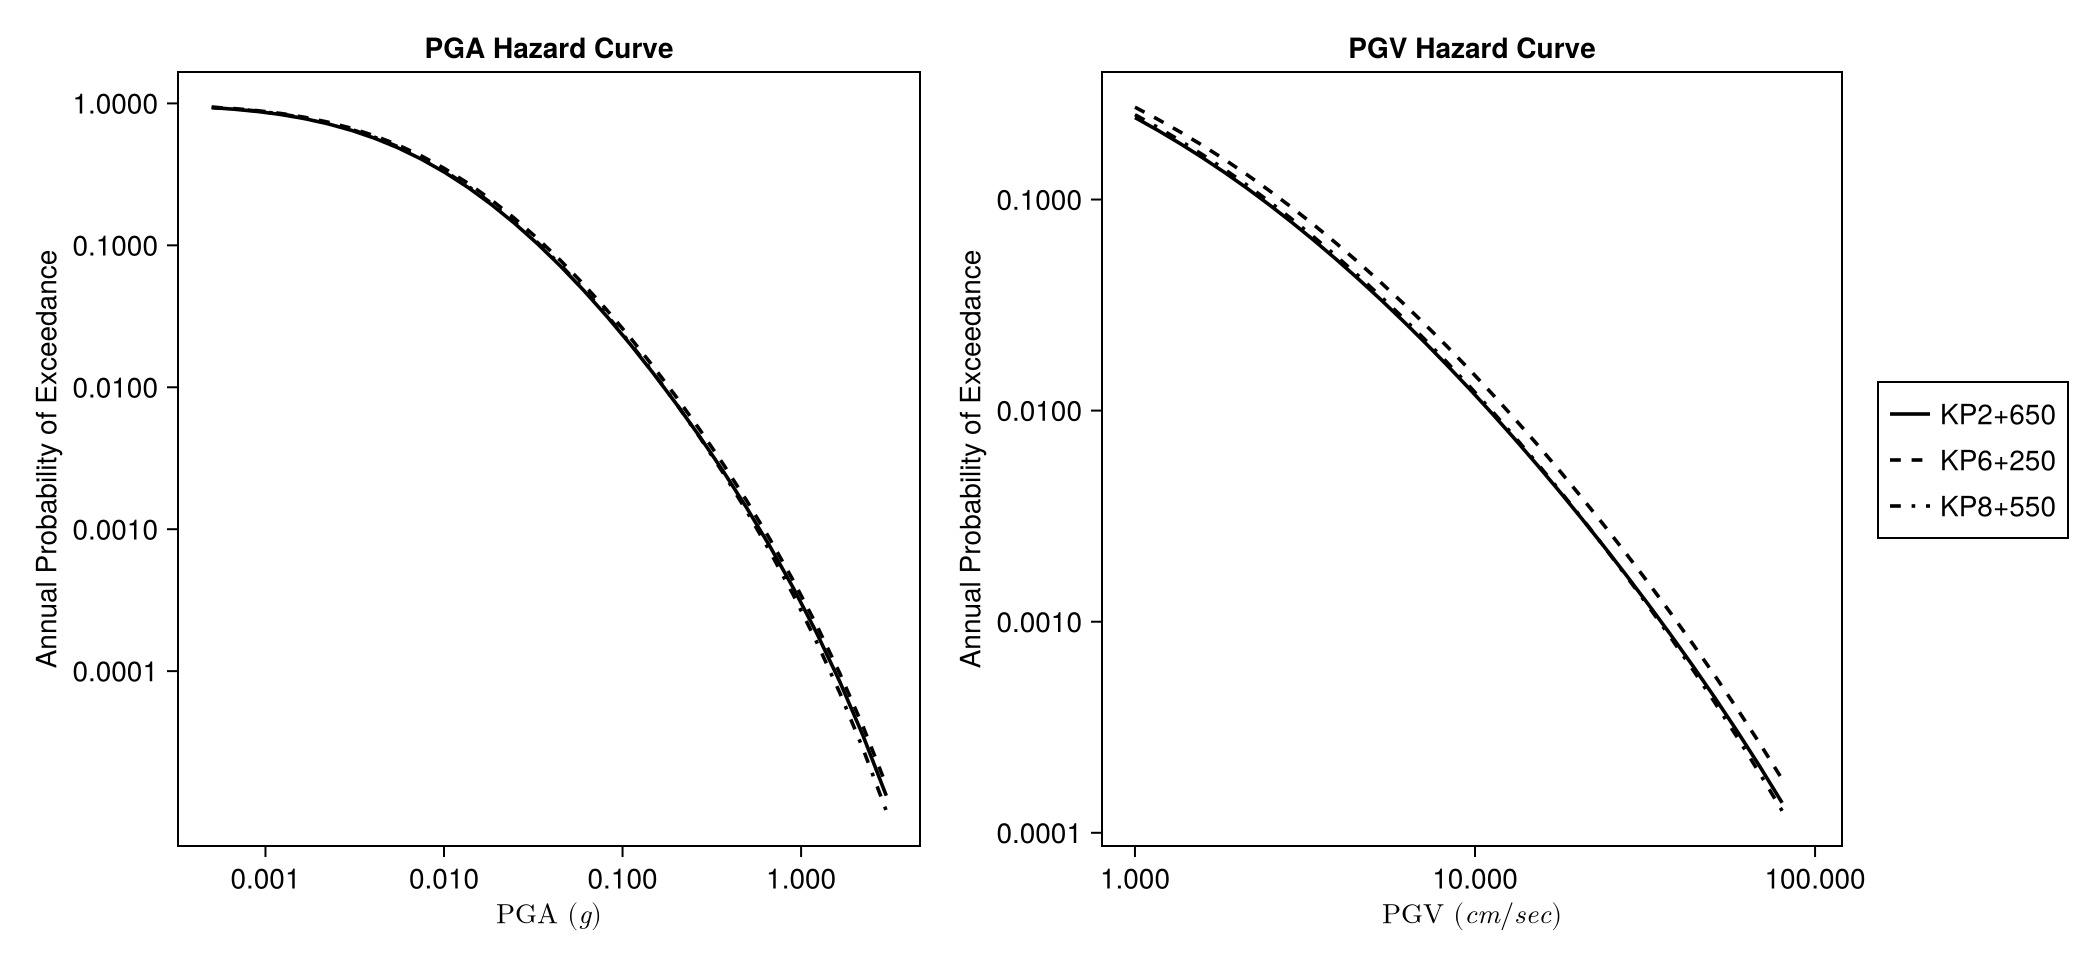
\includegraphics[width=1.05\linewidth]{figures/hazard/hazard-curves.png}
	\caption{Καμπύλες Επικινδυνότητας}
	\label{fig:hcs}
\end{figure}


Εννοείται οι καμπύλες δεν έχουν μεγάλες διαφορές σε τιμές, αλλά η βασικότερη τους χρηιμότητα είναι η παραγωγή της διακινδύνευσης στο τέλος, άρα η διακύμανση των τιμών κατά μήκος του άξονα της γραμμής ευνοεί που είναι σημαντικά μικρή και μπορεί εύκολα να προσεγγιστεί μία μέση τιμή.

\subsection{Χάρτες Επικινδυνότητας}
Τα σημαντικότερα αποτελέσματα, και τα πλέον χρηστικά, παρουσιάστηκαν στις προηγούμενες υποενότητες. Στην παρούσα ενότητα τοποθετούνται οι χάρτες επικινδυνότητας που παρήχθησαν, οι οποίοι δεν έχουν τόση υπολογιστική αξία, όσο είναι χρήσιμη για ποιοτική αποτύπωση των αποτελεσμάτων.

Οι χάρτες έχουν πλαίσιο όπως αυτό του Σχήματος \ref{fig:bores}, και όλες οι τιμές λαμβάνονται για σεισμικά γεγονότα με περίοδο αναφοράς 2500 έτη 


\begin{minipage}{1.15\linewidth}
	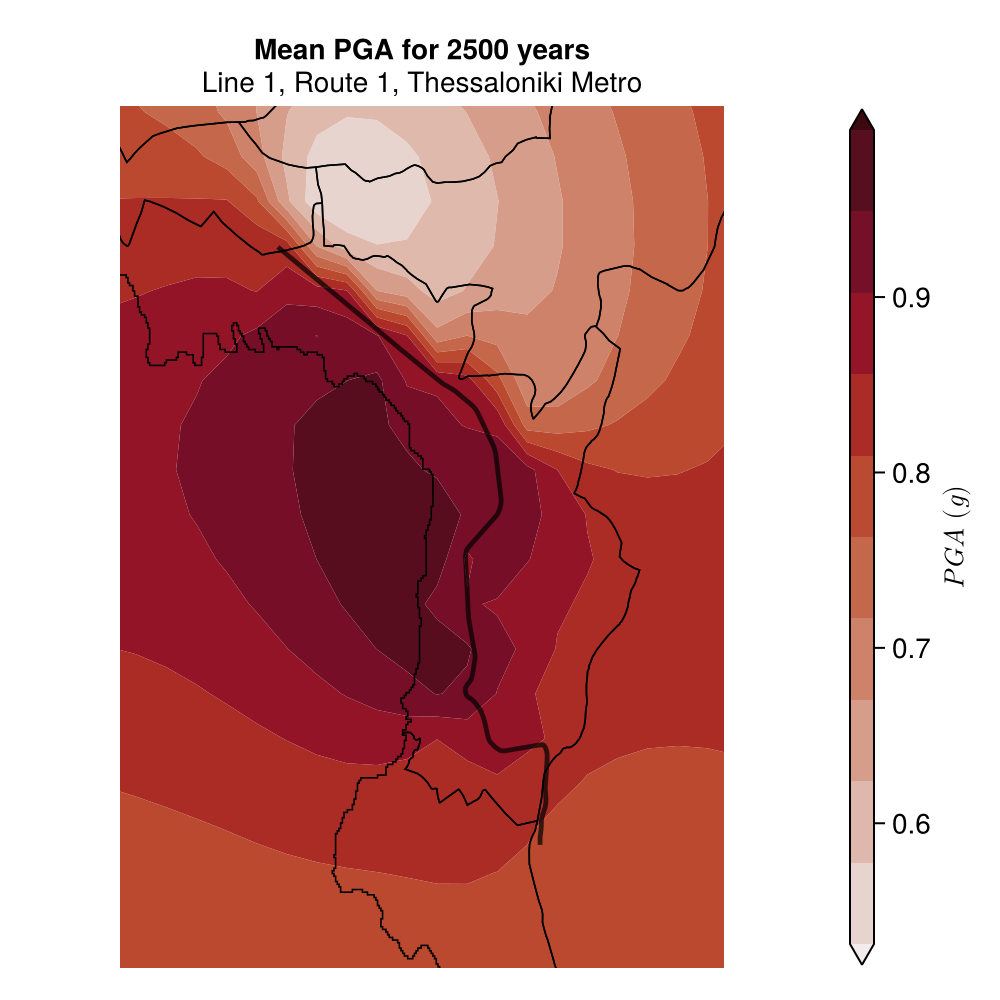
\includegraphics[width=0.5\textwidth]{figures/hazard/Map_measured_PGA.png}
	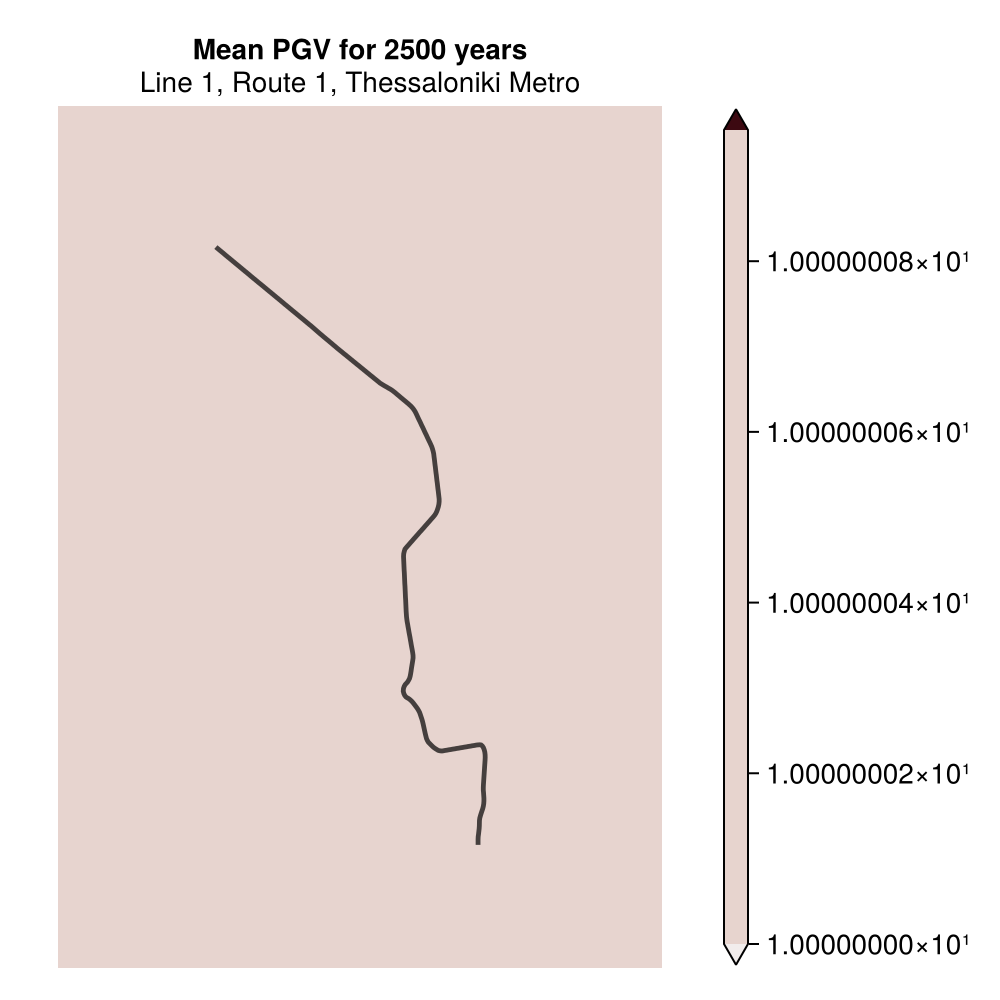
\includegraphics[width=0.5\textwidth]{figures/hazard/Map_measured_PGV.png}
	\captionof{figure}{Χάρτες Μέσων PGA-PGV Γεωτρήσεων}
	\label{fig:maps-m}
\end{minipage}

\begin{minipage}{1.13\linewidth}
	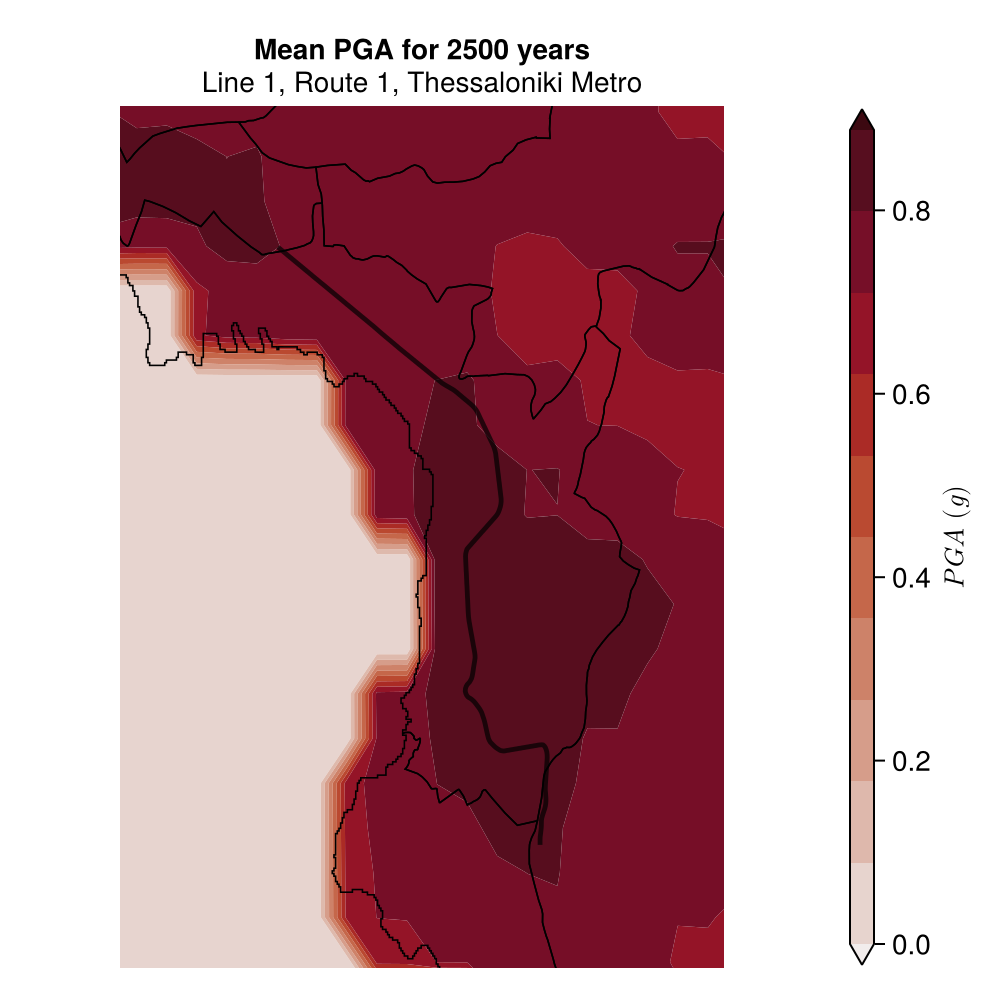
\includegraphics[width=0.5\textwidth]{figures/hazard/Map_assigned_PGA.png}
	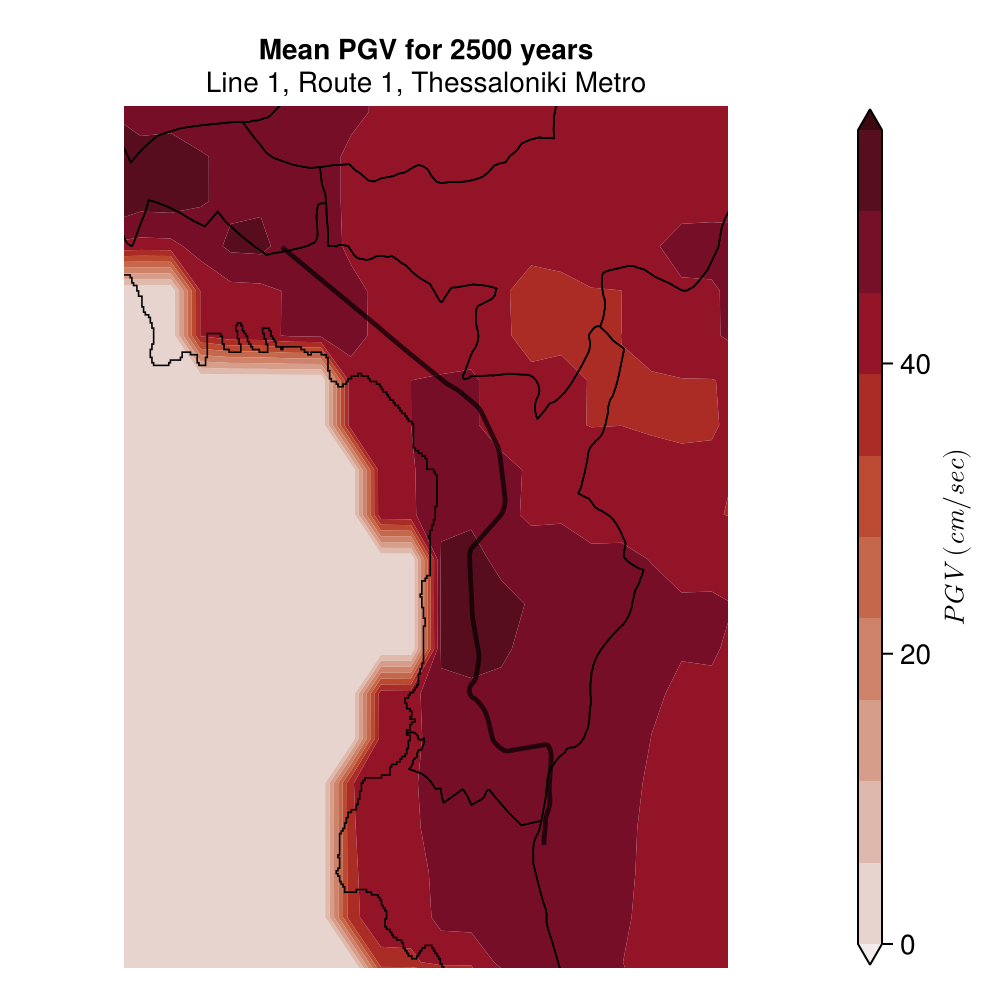
\includegraphics[width=0.5\textwidth]{figures/hazard/Map_assigned_PGV.png}
	\captionof{figure}{Χάρτες Μέσων PGA-PGV $V_{s30}$ ESRM20}
	\label{fig:maps-a}
\end{minipage}

\begin{minipage}{1.13\linewidth}
	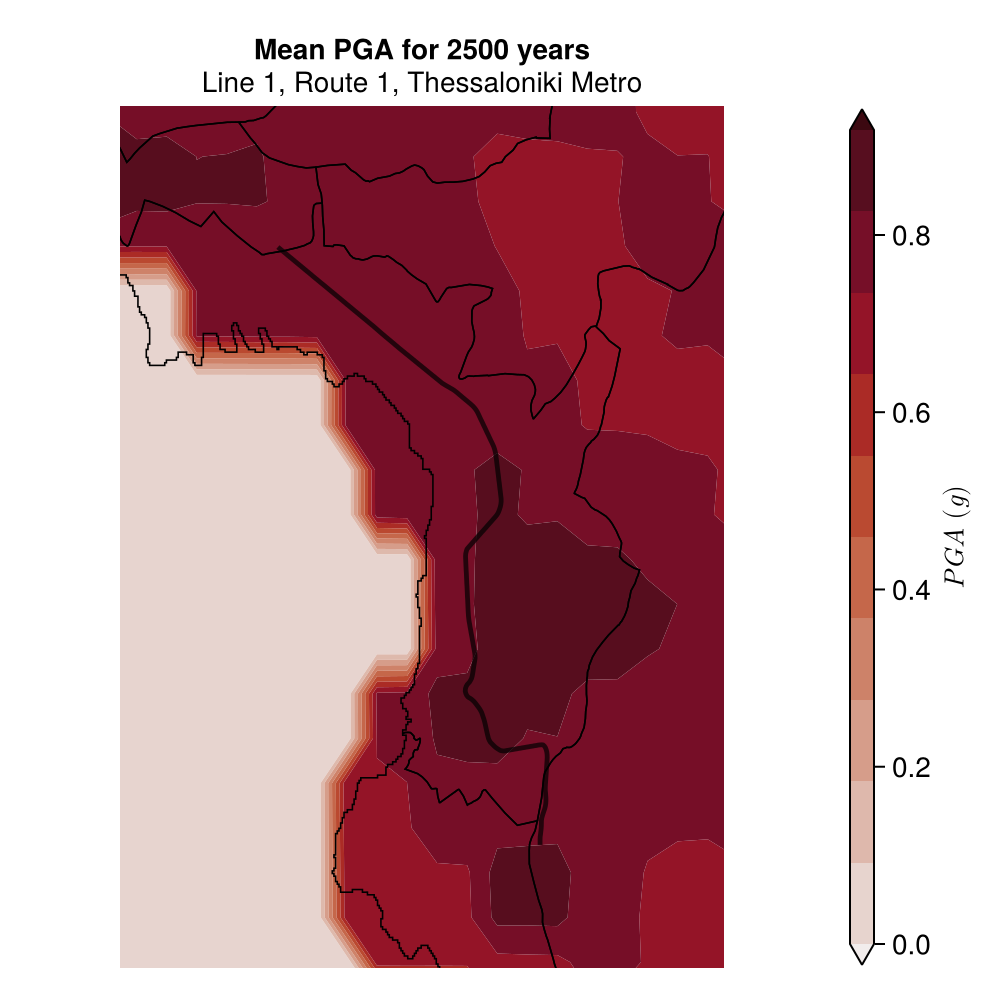
\includegraphics[width=0.5\textwidth]{figures/hazard/Map_slope_PGA.png}
	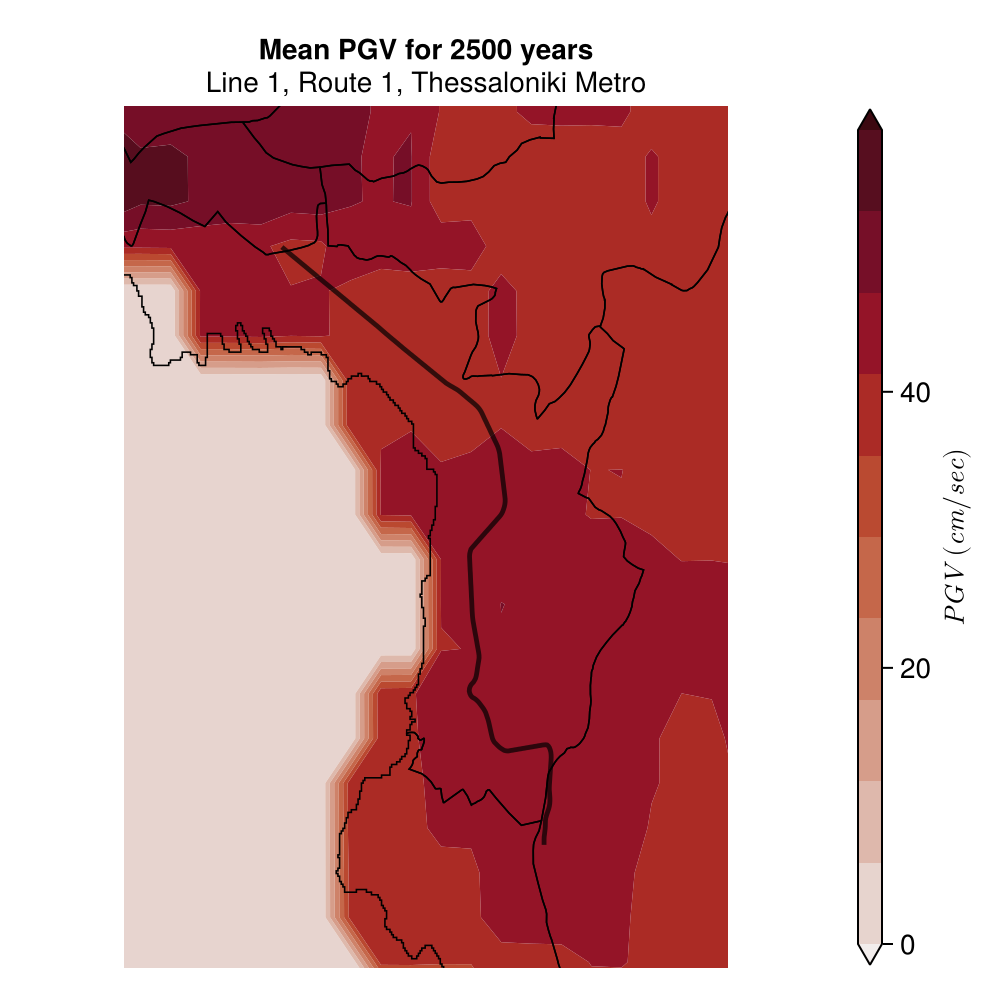
\includegraphics[width=0.5\textwidth]{figures/hazard/Map_slope_PGV.png}
	\captionof{figure}{Χάρτες Μέσων PGA-PGV Γεωλογίας-Κλίσης ESRM20}
	\label{fig:maps-sg}
\end{minipage}



